%--------------------------------------------------------------
% thesis.tex 
%--------------------------------------------------------------
% Corso di Laurea in Informatica 
% - template for the main file of Informatica@Unifi Thesis 
% - based on Classic Thesis Style Copyright (C) 2008 
%   Andr\'e Miede http://www.miede.de   
%--------------------------------------------------------------
\documentclass[twoside,openright,titlepage,
	headinclude,12pt,a4paper,BCOR=5mm,footinclude,bibliography=totoc,listof=totoc]{scrbook}
%--------------------------------------------------------------
% Inputs for the title page 
%--------------------------------------------------------------
\newcommand{\myItalianTitle}{Steganografia generativa su immagini:\\adattamento del protocollo Meteor tramite l'architettura VQ-GAN\xspace}
\newcommand{\myEnglishTitle}{Generative Image Steganography: Adapting the Meteor Protocol to the VQ-GAN Architecture\xspace}
% use the right myDegree option
\newcommand{\myDegree}{Corso di Laurea in Informatica\xspace}
%\newcommand{\myDegree}{Corso di Laurea Magistrale in Informatica\xspace}
\newcommand{\myName}{Matteo Diciotti\xspace}
\newcommand{\mySupervisorTitle}{Relatore\xspace} %%% remove one of the two
\newcommand{\mySupervisorName}{Prof. \textit{Daniele Baracchi}\xspace} 
\newcommand{\myFirstCoSupervisorTitle}{Correlatrice\xspace} %%% optional: remove this command if the thesis has no Co-Supervisor
\newcommand{\myFirstCoSupervisorName}{PhD \textit{Giulia Bertazzini}\xspace} %%% optional: remove this command if the thesis has no Co-Supervisor
\newcommand{\mySecondCoSupervisorTitle}{Correlatore\xspace} %%% optional: remove this command if the thesis has less than 2 Co-Supervisors
\newcommand{\mySecondCoSupervisorName}{Prof. \textit{Daniele Castellana}\xspace} %%% optional: remove this command if the thesis has less then two Co-Supervisors
\newcommand{\myTime}{Anno Accademico 2025-2026\xspace}
%--------------------------------------------------------------

\usepackage[utf8]{inputenc} 
\usepackage[T1]{fontenc} 

% switch italian and english, depending on the language of the thesis
% this will change the chapter titles
\usepackage[italian]{babel}
%\usepackage[english]{babel}
\usepackage{csquotes}	

\usepackage[
	backend    = biber, 
	style      = numeric-comp,
	backref    = true, 
	sorting    = ydnt,
	]{biblatex}
\bibliography{Bibliography} % Entries are in the Bibliography.bib file

\usepackage{amsmath}
\usepackage{mathtools}
\usepackage{ellipsis}
\usepackage{listings}
\usepackage{enumitem}
\usepackage{subfig}
\usepackage{caption}
\usepackage{appendix}
\usepackage{siunitx}
\usepackage{algorithm}
\usepackage{algpseudocode}
\floatname{algorithm}{Algoritmo}
\def\algorithmautorefname{Algoritmo}
\algrenewcommand{\algorithmicrequire}{\textbf{Require:}}
\algrenewcommand{\algorithmicensure}{\textbf{Ensure:}}
% Controllo vedove/orfani: almeno 2 righe alla pagina successiva o nessuna
\clubpenalties=3 600 600 600
\widowpenalties=3 600 600 600
\usepackage[pdftex]{graphicx} 
\graphicspath{{./Figures/}}
\usepackage[eulerchapternumbers,
		    linedheaders,
		    subfig,
		    beramono,
		    eulermath,
		    parts,
		    dottedtoc]{classicthesis}
%--------------------------------------------------------------
% Layout setting
%--------------------------------------------------------------
\newlength{\abcd} 
\newcommand{\myfloatalign}{\centering} 
\setlength{\extrarowheight}{3pt} 
\captionsetup{labelfont=bf, format=plain, font=small, skip=0.5\baselineskip}

\usepackage{geometry}
\geometry{
	a4paper,
	ignoremp,
	bindingoffset = 1cm, 
	textwidth     = 13.5cm,
	textheight    = 21.5cm,
	lmargin       = 3.5cm, 
	tmargin       = 4cm    
}

\lstset{
  	frame=tb,
		language=python,
  	aboveskip=3mm,
  	belowskip=3mm,
  	showstringspaces=false,
  	columns=flexible,
  	basicstyle={\small\ttfamily},
  	numbers=none,
  	breaklines=true,
  	breakatwhitespace=true,
  	tabsize=3
}
\addto\captionsitalian{%
  \renewcommand{\lstlistingname}{Listato}
}
%--------------------------------------------------------------
% Hyperlinks and references setting
%--------------------------------------------------------------
\usepackage{tikz}
\usetikzlibrary{arrows.meta, positioning, shapes.geometric, fit, backgrounds, calc}
\usepackage{hyperref}
\hypersetup{
	colorlinks=true,
	linkcolor=blue,
	filecolor=magenta,      
	urlcolor=cyan,
	pdfpagemode=FullScreen,
	linktoc=all
}
%--------------------------------------------------------------
\begin{document}
\frenchspacing
\raggedbottom
\pagenumbering{roman}
\pagestyle{plain}
%--------------------------------------------------------------
% Frontmatter
%--------------------------------------------------------------
\include{FrontMatter/TitlePage}
\pagestyle{scrheadings}
%--------------------------------------------------------------
% Mainmatter
%--------------------------------------------------------------
\pagenumbering{arabic}
\tableofcontents
\listoffigures
\cleardoublepage
\thispagestyle{empty}
\begin{flushright}
	\null\vspace{\stretch {1}}
	%--------------------------------------------------------------
	% Citation
	%--------------------------------------------------------------
	\emph{"Questo è bello!"\\
		"Eh, nella sua semplicità.."\\
		"Questo è iper-realista."\\
		"E se me lo concedi monocromatico."\\
		"L'artista è Meteor."\\
		"Meteor, già sentito!"\break --- Aldo, Giovanni e Giacomo} \vspace{\stretch{2}}\null
\end{flushright}
\cleardoublepage

%--------------------------------------------------------------
% Chapters
%--------------------------------------------------------------
% !TEX root = ../Thesis.tex

\chapter{Introduzione}
L'esigenza intrinseca e crescente di garantire comunicazioni che siano contemporaneamente riservate, autentiche e integre rappresenta un pilastro fondamentale su cui si erge l'architettura stessa del mondo digitale contemporaneo. La sicurezza delle informazioni, in passato, è stata prevalentemente affidata a robuste tecniche crittografiche e a protocolli standard ben consolidati, quali il Transport Layer Security (TLS) e il suo predecessore Secure Sockets Layer (SSL). Questi sistemi sono stati meticolosamente progettati per rendere il contenuto effettivo dei messaggi inaccessibile a qualsiasi entità esterna non in possesso delle chiavi di decifratura appropriate; nel contesto di TLS, ciò si traduce tipicamente nell'esclusione di chiunque non partecipi al processo di negoziazione della connessione (l'handshake).

Tuttavia, l'escalation senza precedenti delle misure di sorveglianza di massa su scala globale e la proliferazione di meccanismi di censura sempre più capillari e sofisticati hanno messo a nudo una vulnerabilità critica, intrinseca e finora difficile da eradicare alla crittografia moderna: la sua stessa visibilità. Sebbene la crittografia riesca efficacemente a mantenere segreto il contenuto dei dati trasmessi, l'elevata entropia e le caratteristiche distintive del traffico cifrato lo rendono facilmente identificabile e distinguibile dalle comunicazioni in chiaro. Questo stato di cose consente a regimi autoritari, a entità statali o a sofisticati sistemi di filtraggio di rete (come i firewall avanzati) di individuare, bloccare o degradare selettivamente le comunicazioni protette, compromettendo così l'effettivo scambio di informazioni sensibili in contesti operativi ostili o sorvegliati.

Di fronte a tali sfide, specialmente in scenari caratterizzati da censura estrema o da ambienti di comunicazione altamente avversari, emerge in modo prepotente la necessità di esplorare e impiegare metodologie steganografiche. La steganografia, come disciplina, si dedica all'arte e alla scienza dell'occultamento di informazioni segrete all'interno di oggetti di copertura (cover objects) che, a un'osservazione superficiale, appaiono del tutto innocui e non sospetti. Questi oggetti di copertura possono assumere svariate forme, tra cui testi, immagini, file audio o video. A differenza della crittografia, il cui successo e la cui sicurezza dipendono in larga misura dalla complessità matematica o computazionale necessaria per decifrare il messaggio cifrato, la sicurezza in ambito steganografico poggia su un principio radicalmente diverso: l'indistinguibilità statistica. L'obiettivo primario è fare in modo che un osservatore esterno non sia minimamente in grado di discriminare tra un oggetto che contiene un messaggio segreto (denominato stego-object) e un oggetto analogo che ne è privo.

Le metodologie steganografiche classiche, quali ad esempio la manipolazione dei bit meno significativi (Least Significant Bit - LSB) nelle immagini digitali, si sono progressivamente rivelate vulnerabili agli attacchi di crittoanalisi statistica sempre più avanzati e raffinati. Per superare queste limitazioni intrinseche e garantire un livello di sicurezza che sia non solo robusto ma anche dimostrabile, la ricerca più recente ha abbracciato un vero e proprio cambio di paradigma. Questo nuovo orientamento si concentra sull'utilizzo strategico di modelli generativi, in particolare quelli basati su reti neurali profonde.

In questo fertile contesto di ricerca si inserisce \textbf{Meteor}, un innovativo algoritmo di steganografia a chiave simmetrica. Meteor sfrutta le potenti capacità computazionali e generative dei modelli di linguaggio di grandi dimensioni (Large Language Models - LLM), originariamente derivati da architetture come GPT-2, per creare canali di comunicazione occulti e resilienti. A differenza delle tecniche steganografiche tradizionali che modificano un contenuto esistente, Meteor interviene e guida il processo di generazione stessa del contenuto. Esso utilizza la distribuzione di probabilità intrinseca del modello generativo per "pilotare" il campionamento dei token successivi in base al messaggio segreto opportunamente cifrato. Questo approccio garantisce che lo stego-object risultante sia statisticamente coerente e indistinguibile dall'output naturale del modello, rendendo la presenza del messaggio nascosto estremamente difficile, se non impossibile, da rilevare attraverso analisi statistiche convenzionali.

L'ambizioso obiettivo della presente tesi triennale è estendere il principio fondamentale di sicurezza steganografica ideato da Meteor, originariamente applicato al dominio testuale, all'ambito delle immagini digitali ad alta risoluzione.
Per conseguire questo scopo, viene sfruttata l'architettura \textbf{VQ-GAN} (Vector Quantized Generative Adversarial Network). La scelta strategica di questa specifica architettura deriva dalla sua intrinseca capacità di modellare immagini estremamente complesse attraverso la creazione e l'utilizzo di un vocabolario discreto di "token visivi", memorizzati in un codebook. Questa rappresentazione discreta apre le porte all'applicazione di un modello Transformer autoregressivo, ampiamente utilizzato nella generazione sequenziale, per guidare il processo di sintesi dell'immagine.
Il lavoro svolto mira dunque a dimostrare con rigore e sperimentazione come sia possibile incorporare messaggi cifrati direttamente durante la fase di generazione dell'immagine da parte dell'architettura VQ-GAN. L'obiettivo finale è ottenere immagini non solo visivamente simili a quelle generate dalla stesso modello, ma anche intrinsecamente robuste contro tentativi sofisticati di rilevamento steganografico.

Le implicazioni pratiche e teoriche di questo approccio sono potenzialmente rivoluzionarie per lo sviluppo di strumenti di comunicazione \emph{censorship-resistant}. La capacità di abilitare lo scambio sicuro e nascosto di informazioni all'interno di immagini di alta qualità offre un livello inedito di protezione per la privacy degli utenti e per la libertà di espressione in contesti digitali sempre più soggetti a sorveglianza e controllo.

\bigskip

Il presente elaborato è stato organizzato con cura per condurre il lettore attraverso un percorso logico e approfondito, dalla teoria alla pratica:

\begin{itemize}
	\item Il \textbf{\autoref{ch:stato-arte}} fornisce un'analisi completa e dettagliata del background teorico indispensabile, approfondendo lo stato dell'arte delle tecniche steganografiche esistenti e i principi fondamentali di funzionamento dei modelli generativi più avanzati, con un'enfasi particolare sulle architetture GAN (Generative Adversarial Networks) e Transformer.
	\item Il \textbf{\hyperref[cap-3]{Capitolo 3}} presenta le definizioni formali e le specifiche tecniche del sistema proposto, illustrando in dettaglio l'architettura implementata e le modifiche apportate al meccanismo di campionamento dei token visivi per consentire l'embedding del messaggio segreto cifrato direttamente nel flusso generativo. Vengono inoltre discussi i limiti teorici e pratici del lavoro svolto, evidenziando le sfide affrontate e le soluzioni adottate per superarle.
	
	\item Il \textbf{\hyperref[cap-4]{Capitolo 4}} presenta l'idea alla base del lavoro di tesi,l'architettura completa del sistema implementato e i limiti teorici e pratici del lavoro svolto. Vengono illustrate in dettaglio le modifiche apportate al meccanismo di campionamento dei token visivi per consentire l'embedding del messaggio segreto cifrato direttamente nel flusso generativo.
	
	\item Il \textbf{\hyperref[cap-5]{Capitolo 5}} espone in modo esaustivo i risultati delle sperimentazioni condotte. Vengono valutate sia la qualità visiva delle immagini generate, attraverso l'utilizzo di metriche consolidate come la Fréchet Inception Distance (FID), sia la capacità steganografica del sistema, analizzando il payload trasferibile e la robustezza contro attacchi di rilevamento.
	
	\item Infine, il \textbf{\hyperref[cap-6]{Capitolo 6}} trae le conclusioni finali del lavoro svolto, riassumendo i contributi principali della ricerca e delineando una serie di possibili sviluppi futuri, mirati al miglioramento incrementale dell'efficienza, della robustezza e della sicurezza complessiva del sistema proposto.
\end{itemize}
% !TEX root = ../Thesis.tex

\chapter{Stato dell'arte}\label{ch:stato-arte}

\section[Meteor]{Meteor: un framework di steganografia generativa su testo}

\subsection{Contesto e motivazioni}
La necessità di una solida comprensione teorica, indispensabile per contestualizzare appieno il presente lavoro di ricerca, si articola attraverso una costellazione di concetti interdipendenti che convergono in un'unica opera fondamentale: il lavoro di \cite{kaptchuk-2021}, comunemente noto come \emph{Meteor}. Questa pionieristica indagine, che va oltre una mera disamina della steganografia classica e di quella generativa, introduce primariamente un approccio metodologico e, in secondo luogo, un framework robusto ed efficiente deputato alla \emph{generazione di messaggi testuali contenenti informazioni celate}.

La peculiarità di queste informazioni risiede nella loro intrinseca invisibilità non solo all'occhio umano, ma anche, e soprattutto, alle più sofisticate tecniche di steganalisi basate su divergenza statistica. La ragione di tale elusività risiede nella formalizzazione del concetto di \emph{perfectly secure steganography} nel dominio del linguaggio naturale: il testo generato da \emph{Meteor} non manifesta alcuna deviazione statistica significativa rispetto a un testo prodotto autonomamente dal medesimo modello linguistico di base (il cosiddetto \emph{cover distribution}). Come verrà dettagliato in seguito, \emph{Meteor} si avvale di un modello linguistico che ha raggiunto una notevole notorietà, estendendosi ben oltre gli ambiti accademici tradizionali, configurandosi come uno dei primi Transformer a larga scala a influenzare il dibattito pubblico sulla capacità generativa delle IA. Nello specifico, \emph{Meteor} impiega il modello \textbf{GPT-2} (Generative Pre-trained Transformer 2), caratterizzato da un'architettura \emph{decoder-only} addestrata su un corpus massivo di dati testuali (WebText). Tuttavia, l'architettura del framework è stata concepita con una notevole flessibilità, risultando agnostica rispetto al modello linguistico sottostante (\emph{Backbone LLM}). Questa modularità permette a \emph{Meteor} di beneficiare direttamente dei progressi nello stato dell'arte dei modelli linguistici, poiché l'efficacia della steganografia è intrinsecamente legata alla capacità del modello di approssimare la vera distribuzione del linguaggio umano ($P_{data}$).

Per una comprensione ancora più profonda, è opportuno esaminare il contesto socio-tecnologico in cui \emph{Meteor} è maturato e le problematiche specifiche che si proponeva di risolvere, con particolare attenzione alla crescente sofisticazione dei sistemi di sorveglianza e censura digitale. In un'epoca in cui la libertà di espressione e la privacy online sono costantemente minacciate da regimi autoritari e da sistemi di filtraggio sempre più avanzati, la necessità di strumenti di comunicazione \emph{censorship-resistant} è diventata più urgente che mai. \emph{Meteor} si inserisce in questo contesto come una risposta innovativa, offrendo un metodo per nascondere informazioni all'interno di testi generati in modo naturale, rendendo estremamente difficile per qualsiasi osservatore esterno rilevare la presenza di un messaggio segreto.

L'essenza di \emph{Meteor} risiede nell'idea innovativa di utilizzare un modello generativo per la creazione di contenuti steganografici, sfruttando la sua capacità di modellare la probabilità condizionata $P(x_t | x_{<t})$. In termini pratici, il modello agisce come un sofisticato stimatore di densità: data una sequenza di contesto iniziale (\emph{prompt}), esso fornisce una distribuzione di probabilità dettagliata (solitamente tramite una funzione \emph{softmax} applicata ai \emph{logits}) per tutti i possibili \emph{token} contenuti nel vocabolario $\mathcal{V}$. La scelta del \emph{token} da inserire nella sequenza viene effettuata tramite un meccanismo di campionamento che mappa i bit del messaggio segreto in indici del vocabolario, seguendo l'ordinamento indotto dalla distribuzione di probabilità. Questa metodologia trasforma il processo di inferenza in un'operazione di codifica di canale: il testo risultante è statisticamente probabile secondo il modello, ma contiene un messaggio segreto decodificabile univocamente dal destinatario. La decodifica è resa possibile a condizione che il ricevente disponga dello stesso modello linguistico, della medesima sequenza di contesto e di una chiave privata condivisa (\emph{shared secret}), necessaria per inizializzare il generatore di numeri pseudo-casuali o per definire le permutazioni degli indici del vocabolario.

Costruiamo ora uno scenario illustrativo volto a consolidare la comprensione del meccanismo operativo di \emph{Meteor}. Immaginiamo una comunicazione confidenziale tra due entità, Alice ($A$) e Bob ($B$), che desiderano scambiarsi informazioni sensibili attraverso un canale pubblico monitorato. L'obiettivo primario è impedire a un osservatore avversario, Eve ($E$), di rilevare la presenza stessa della comunicazione (\emph{steganographic undetectability}). Un contesto critico si verifica quando Alice o Bob operano all'interno di infrastrutture soggette a \emph{Deep Packet Inspection} (DPI) o filtraggio governativo stringente. In tali scenari, i messaggi cifrati tramite crittografia standard (come AES o RSA) presentano un'elevata entropia e caratteristiche distintive che li rendono facilmente identificabili come traffico cifrato, risultando facilmente identificabili come traffico non lecito e quindi soggetto a blocco immediato (\autoref{fig:alice-bob-eve-firewall}). Un esempio emblematico è il sistema descritto in \autocite{chinawall-2015}, il "\emph{Great Firewall}", che impiega euristiche avanzate per discriminare tra traffico legittimo e protocolli di tunneling o cifratura.
All'interno di questo quadro ostile, la steganografia generativa supera il limite della crittografia tradizionale: non si limita a proteggere il contenuto, ma nasconde l'esistenza stessa dell'atto comunicativo. Eve, osservando il transito di un testo coerente e stilisticamente appropriato, non ha basi statistiche per etichettare la comunicazione come sospetta\footnote{Nel presente scenario, "segreto" e "privato" sono usati in senso tecnico: una comunicazione è steganograficamente sicura se la divergenza di Kullback-Leibler tra la distribuzione dei messaggi naturali e quella dei messaggi steganografici tende a zero.}.

\begin{figure}[tbh]
	\centering
	\frame{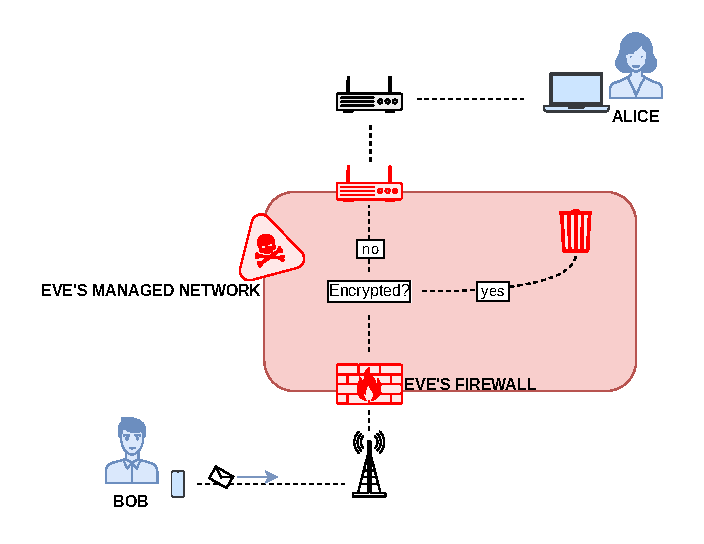
\includegraphics[width=.8\textwidth]{AliceBobEveFirewall.pdf}}
	\caption[Alice e Bob attraversano il firewall di Eve]{Rappresentazione schematica di una comunicazione tra Alice (A) e Bob (B) in presenza di un osservatore esterno, Eve (E), e di un sistema di filtraggio dei contenuti (Firewall) che analizza la firma statistica dei pacchetti.}
	\label{fig:alice-bob-eve-firewall}
\end{figure}

Sotto il profilo teorico, la progettazione di \emph{Meteor} ha richiesto la risoluzione di due criticità fondamentali intrinseche alla natura del linguaggio naturale.

La prima sfida concerne la definizione di un \emph{sampler steganografico} efficace. L'algoritmo deve mappare il contesto fornito al modello in una distribuzione di probabilità del token successivo che ricalchi quanto più fedelmente possibile quella del linguaggio naturale. Risulta tuttavia evidente che il linguaggio naturale non sottostia a una distribuzione di probabilità assoluta e invariante: si considerino, a titolo esemplificativo, le divergenze linguistiche intercorrenti tra un testo dei primi del Novecento e uno contemporaneo, o tra la prosa scientifica e quella letteraria. \emph{Meteor} affronta tale complessità adottando un modello di generazione testuale come approssimatore dinamico del linguaggio naturale. Tale approccio consente di simulare efficacemente la distribuzione linguistica in molteplici domini, superando il problema dell'assenza di una distribuzione statistica universale che ha storicamente limitato la steganografia classica. È tuttavia opportuno precisare che l'efficacia di \emph{Meteor} è intrinsecamente dipendente dalla capacità del modello linguistico sottostante (il \emph{Backbone LLM}) di approssimare la distribuzione reale. Qualora il modello non riuscisse a catturare le sfumature e le complessità semantiche del linguaggio umano, la steganografia generativa diverrebbe vulnerabile a tecniche di rilevamento avanzate. Cionondimeno, ogni output prodotto da \emph{Meteor} risulta statisticamente indistinguibile da un testo generato autonomamente dal medesimo modello; ciò garantisce una sicurezza steganografica assoluta, a condizione che non sia possibile distinguere tra un testo prodotto dal modello e uno naturale.

La seconda sfida è legata alla variabilità dell'entropia testuale. In segmenti caratterizzati da elevata densità semantica o vincoli sintattici stringenti (bassa entropia), la libertà di selezione del token successivo è pressoché nulla. Ad esempio, data la sequenza \emph{"The largest carnivore of the Cretaceous period was the Tyrannosaurus"}, il "token" \emph{"Rex"} presenta una probabilità estremamente elevata. Forzare la codifica di bit in tale posizione selezionando un token alternativo produrrebbe un'anomalia semantica macroscopica, facilmente individuabile da un classificatore neurale. Per ovviare a ciò, \emph{Meteor} introduce una soglia di entropia minima: il sistema analizza la distribuzione di probabilità a ogni passo temporale e determina dinamicamente se la varianza sia sufficiente per ospitare informazione. Se l'entropia è inferiore a un valore critico $\tau$, il sistema genera un token senza inserire informazione steganografica. Qualora, invece, l'entropia superi tale soglia, il sistema seleziona i token con probabilità rilevante, escludendo la coda della distribuzione. Attraverso un meccanismo di partizionamento degli indici basato sulle probabilità relative, viene campionato il token i cui estremi dell'intervallo di probabilità presentino una corrispondenza tra i bit più significativi e i bit del messaggio da codificare. Nel caso in cui l'intervallo non permetta la codifica di alcun bit (ovvero quando gli estremi non condividono il prefisso binario), \emph{Meteor} adotta una strategia a bitrate variabile, rinunciando all'inserimento di informazione per quel determinato passo. In fase di decodifica, la conoscenza della distribuzione di probabilità e dei relativi indici consente di determinare univocamente se l'informazione sia stata inserita o meno, potendo recuperare l'intervallo relativo al token selezionato e recuperando i bit più significativi comuni per tutti i valori nell'intervallo. Sebbene tale eventualità sia rara data l'elevata entropia media del linguaggio, questa strategia di codifica adattiva (\emph{adaptive rate}) garantisce che il throughput informativo sia massimizzato esclusivamente dove il linguaggio offre una ridondanza naturale, preservando rigorosamente l'integrità statistica del testo prodotto.

\subsection{Meccanismo Operativo del Protocollo Meteor}

Il concetto fondamentale che differenzia Meteor dai metodi tradizionali di steganografia è lo spostamento del paradigma: l'informazione non viene "nascosta" all'interno di un oggetto esistente tramite modifiche (embedding), ma viene utilizzata per \textbf{guidare il processo di campionamento} durante la generazione di un nuovo media.

Il funzionamento pratico del protocollo si articola nelle seguenti fasi sequenziali:

\begin{enumerate}
	\item \textbf{Cifratura del Messaggio:} Il messaggio segreto viene cifrato utilizzando una chiave simmetrica condivisa tra mittente e destinatario. Questo passaggio è essenziale per trasformare il messaggio in una stringa di bit computazionalmente indistinguibile dal rumore casuale, garantendo che le scelte di campionamento effettuate dal protocollo non presentino pattern statistici rilevabili.

	\item \textbf{Accesso alla Distribuzione Condizionata:} Meteor si appoggia a un modello generativo pre-addestrato (originariamente GPT-2 il quale possiede un'architettura basata su Transformers, necessità imprescindibile anche per lo sviluppo di modelli nel dominio visivo, quindi anche nel caso della VQ-GAN utilizzata nella nostra implementazione, che vedremo in seguito). Ad ogni passo temporale $t$, il modello riceve il contesto dei token già generati e produce una \textbf{distribuzione di probabilità $P$} su tutto il vocabolario dei possibili token successivi.

	\item \textbf{Campionamento Vincolato:} Invece di campionare casualmente o scegliere il token più probabile, Meteor utilizza i bit del messaggio cifrato come "indice" per selezionare il token dalla distribuzione $P$. Lo spazio di probabilità viene partizionato e mappato sulle sequenze di bit in modo che il token scelto sia sempre \textbf{statisticamente coerente} con il modello, selezionando il token tra quelli più probabili, eliminando la coda della distribuzione sotto una soglia pre-specificata di probabilità. Poiché la scelta avviene all'interno della distribuzione naturale del modello, l'output steganografico rimane indistinguibile da un output generato classicamente dallo stesso modello.

	\item \textbf{Generazione Iterativa:} Questo processo avviene in modo autoregressivo. Ogni token generato entra a far parte del nuovo contesto per il passo successivo, continuando fino a quando l'intero media (o la sequenza di token visivi necessari per ricostruire l'immagine tramite il decoder VQ-GAN) non è completo. Il troncamento non è netto dopo la codifica dell'ultimo token, ma può essere definito da un carattere speciale che indica la fine del messaggio, o da un limite di lunghezza predefinito. In questo modo, il testo o l'immagine risultante è completamente naturale e coerente, senza alcuna evidenza della presenza di un messaggio nascosto.

	\item \textbf{Estrazione e Decodifica:} Il ricevente, possedendo lo stesso modello generativo e la chiave simmetrica, è in grado di ricreare le medesime distribuzioni di probabilità $P$ per ogni passo del processo. Identificando quali token sono stati effettivamente inclusi nello stego-media ricevuto, il destinatario può risalire ai bit che hanno determinato quelle scelte, ricostruendo il messaggio cifrato e, infine, il segreto originale.
\end{enumerate}

L'efficacia di Meteor risiede nella sua capacità di eliminare le anomalie statistiche che gli strumenti di \textbf{steganalisi moderna} solitamente identificano. In questo contesto, il messaggio segreto non è contenuto "nei" dati, ma rappresenta la \textbf{ragione deterministica} per cui determinati dati coerenti sono stati generati al posto di altri.

Per comprendere appieno il flusso del protocollo, è utile illustrare uno scenario concreto\footnote{L'esempio proposto rappresenta una forzatura narrativa volta a evitare i classici scenari di sorveglianza bellica o regimi autoritari. Sebbene la trama possa apparire singolare, ogni passaggio tecnico descritto riflette operazioni realmente attuabili a livello pratico.}. Supponiamo che Alice voglia comunicare con il compagno Bob senza che sua madre Eve, esperta di reti di telecomunicazioni e ostile alla loro relazione, lo venga a sapere. Alice ha dimenticato il proprio computer a casa di Bob e deve chiedergli di riportarglielo, ma Eve intercetta ogni comunicazione all'interno della rete domestica. In questo scenario, Alice ha esaurito il traffico dati cellulare e non ha accesso a reti Wi-Fi alternative. Il firewall di casa è stato configurato da Eve per bloccare qualsiasi traffico crittografato end-to-end; i messaggi devono transitare in chiaro per poter superare il gateway. La navigazione esterna è mediata da un proxy che instrada le informazioni tramite un protocollo, ideato dalla stessa Eve, che lascia i contenuti leggibili. Di conseguenza, ogni messaggio inviato o ricevuto da Alice è potenzialmente visibile a sua madre.

In questo contesto, qualsiasi comunicazione cifrata in forma tradizionale verrebbe immediatamente bloccata. Alice e Bob decidono quindi di utilizzare \emph{Meteor}. Alice redige un messaggio segreto: \enquote{Mi porteresti il portatile domani per favore, l'ho lasciato sul tavolo di cucina da te.}. Utilizzando una chiave simmetrica condivisa (ad esempio la data del loro anniversario), Alice cifra il testo ottenendo una stringa di bit. Il messaggio originale, lungo 87 caratteri in codifica ASCII, corrisponde a 87 byte, ovvero 696 bit. Dopo la cifratura, si ottiene una sequenza di 696 bit che è computazionalmente indistingubile da una stringa interamente casuale. Poiché l'invio diretto di tale stringa verrebbe intercettato e bloccato da Eve, Alice si affida a \emph{Meteor} per trasformarla.

Eve è abituata a vedere Alice e Bob scambiarsi testi generati da modelli linguistici mentre studiano insieme per l'università. Alice, studentessa di ingegneria informatica, decide di sfruttare questa abitudine: sa che Eve non sospetterà nulla se vedrà transitare nella chat una serie di messaggi relativi alla preparazione dell'esame di Analisi II, scambiandoli per normali interazioni con un LLM. Alice inserisce il messaggio cifrato in \emph{Meteor} e fornisce come contesto iniziale (\emph{prompt}) il testo di un esercizio sullo studio del dominio di una funzione. Il framework genererà un testo che non solo nasconde il messaggio cifrato in modo trasparente, ma risulterà anche semanticamente coerente con il contesto matematico fornito.

L'efficienza di questo processo dipende dalla \enquote{precisione} di \emph{Meteor}, ovvero dal numero di bit che possono essere codificati in un singolo token. Questo valore è influenzato dalla dimensione del vocabolario e dalla distribuzione di probabilità dei token. Mentre per modelli come GPT-2 è teoricamente possibile codificare fino a 32 bit per token, in media se ne ottengono circa 15. Tuttavia, in contesti a bassa entropia come un esercizio di analisi, la capacità di codifica può scendere sensibilmente. Supponendo uno scenario cautelativo con una capacità di 5 bit per token (con token mediamente composti da 4 caratteri), per codificare i 696 bit del messaggio Alice dovrà generare un testo di circa 140 token (circa 560 caratteri). Tale lunghezza è perfettamente compatibile con una normale risposta di un assistente virtuale.

Per segnalare la fine della comunicazione, può essere utilizzato un carattere speciale che indichi al destinatario il termine del messaggio, per quanto non sia fondamentale in quanto, in caso di assenza di questo carattere, la decodifica procederà normalmente con l'unica differenza che i token decodificati nella fase finale del messaggio sembreranno casuali.

L'output che Eve osserverà sarà simile al seguente:
\begin{lstlisting}[caption={Esempio di testo generato da Meteor contenente un messaggio cifrato. Il messaggio è in formato Markdown, il principale stile di formattazione degli LLM moderni.}, captionpos=b, label={lst:meteor-output-example}]
"Il dominio di una funzione di due variabili e' l'insieme delle coppie $(x, y) \in \mathbb{R}^2$ per le quali la funzione e' definita. Consideriamo ad esempio $f(x, y) = \sqrt{1 - x^2 - y^2}$; affinche' la radice quadrata sia definita, deve valere $1 - x^2 - y^2 \ge 0$, ovvero $x^2 + y^2 \le 1$, che rappresenta il cerchio unitario chiuso nel piano cartesiano. Prendiamo invece $g(x, y) = \frac{1}{x^2 + y^2 - 1}$: il denominatore si annulla quando $x^2 + y^2 = 1$, quindi il dominio e' tutto $\mathbb{R}^2$ esclusa la circonferenza di raggio~1. Per $h(x, y) = \log(x - y)$, la condizione e' $x - y > 0$, ossia il semipiano al di sopra della bisettrice $y = x$. In generale, per determinare il dominio di una funzione multivariata, dobbiamo identificare tutte le condizioni che potrebbero rendere l'espressione non definita, come radici di indice pari di argomenti negativi, denominatori nulli o argomenti di logaritmi non positivi. La soluzione e' tipicamente un sottoinsieme di $\mathbb{R}^2$ o $\mathbb{R}^3$, la cui rappresentazione grafica risulta spesso essenziale per visualizzare le regioni di validita' della funzione."
\end{lstlisting}

In questo testo, i token non sono stati scelti tramite un campionamento casuale (\emph{random sampling}) sulla testa della distribuzione, ma tramite la codifica dei bit del messaggio segreto. Per ogni passo, \emph{Meteor} ha generato la distribuzione di probabilità tramite il modello linguistico, ha rimosso la coda della distribuzione sotto una soglia prefissata e ha ordinato i \emph{logits} ottenuti. Gli indici, distribuiti proporzionalmente alle probabilità dei token in un intervallo da $0$ a $2^p$ (dove $p$ è la precisione), sono stati usati per selezionare il token i cui bit più significativi corrispondessero ai bit successivi del messaggio cifrato.

Se, ad esempio, i bit da codificare fossero \texttt{0101110101...} e le distribuzioni di probabilità dei token disponibili coprissero gli intervalli \texttt{0001...}, \texttt{0100...}, \texttt{0110...} e \texttt{1010...}, \emph{Meteor} selezionerebbe il token associato all'intervallo $[\texttt{0100...}, \texttt{0110...})$, codificando i primi due bit (\texttt{01}). Al passaggio successivo, il token selezionato entra a far parte del contesto del modello e i bit codificati vengono rimossi dalla testa del messaggio segreto, procedendo iterativamente fino al completamento o al raggiungimento dei limiti impostati.

Il testo risultante, coerente e naturale, transita sulla rete domestica senza destare sospetti. Bob, ricevendo il messaggio, utilizza lo stesso modello e la medesima chiave per estrarre i bit e decifrare la comunicazione, comprendendo la richiesta di Alice. Grazie a \emph{Meteor}, Alice è riuscita a eludere la sorveglianza di Eve, rendendo la comunicazione indistinguibile da un comune output di un modello linguistico (e magari è riuscita anche ad ottenere la risposta al problema di analisi che stava studiando, ma questo non dipende da \textit{Meteor}).


\section[VQ-GAN]{VQ-GAN: generazione di immagini ad alta risoluzione}

Successivamente, analizzeremo le ragioni per cui architetture alternative, come le VQ-GAN (Vector Quantized Generative Adversarial Networks), sono state considerate per l'estensione di tali concetti al dominio visuale.

\section{Definizioni e terminologia}

Nel seguito sono presentati un insieme di termini e definizioni fondamentali per la comprensione dei concetti chiave trattati nella tesi. I termini sono organizzati per aree tematiche omogenee, procedendo dai fondamenti della comunicazione sicura fino agli aspetti più specialistici della generazione steganografica. Questo lessico tecnico costituisce il vocabolario essenziale per navigare efficacemente all'interno del discorso sulla steganografia generativa, sui modelli linguistici, sulle architetture di reti neurali e sui generatori di immagini.

\subsection*{Concetti fondazionali della comunicazione}
\begin{itemize}[label=\textbullet, leftmargin=*, itemsep=0em]
	\item \textbf{Plaintext}: locuzione che designa un'informazione nella sua forma originaria e integralmente leggibile, antecedente a qualsiasi trasformazione crittografica o steganografica. Nel contesto della presente trattazione, il plaintext costituisce il dato in chiaro che si intende proteggere.
	\item \textbf{Ciphertext}: denominazione attribuita al risultato dell'applicazione di un algoritmo di cifratura a un plaintext. Tale rappresentazione, strutturalmente incomprensibile in assenza della corrispondente chiave di decifrazione, costituisce il prodotto finale del processo crittografico.
	\item \textbf{Coverobject}: oggetto multimediale originale, nella sua forma inalterata, che funge da contenitore apparentemente innocuo all'interno del quale si intende occultare un messaggio segreto.
	\item \textbf{Stegoobject}: oggetto risultante dall'operazione di incorporazione del messaggio segreto all'interno del coverobject. La proprietà fondamentale che tale artefatto deve soddisfare è l'indistinguibilità percettiva e statistica dal coverobject originale.
	\item \textbf{Payload}: quantità di informazione segreta, espressa in bit, che può essere efficacemente occultata all'interno di un coverobject senza comprometterne l'integrità statistica e percettiva.
\end{itemize}

\subsection*{Discipline della comunicazione sicura}
\begin{itemize}[label=\textbullet, leftmargin=*, itemsep=0em]
	\item \textbf{Crittografia}: disciplina formale che si occupa di rendere non intelligibile un messaggio ad attori non autorizzati mediante l'applicazione di metodi di cifratura. La crittografia costituisce la tecnica preminente per garantire la confidenzialità dei dati nei sistemi informatici contemporanei. Tale disciplina si fonda su principi matematici e algoritmi complessi atti a trasformare l'informazione in una forma cifrata, decifrabile esclusivamente da chi possiede la chiave corretta. La crittografia trova applicazione in molteplici ambiti, tra cui la comunicazione sicura, la protezione dei dati personali e la sicurezza delle transazioni telematiche. Pur costituendo il fondamento dei sistemi comunicativi moderni, la crittografia è potenzialmente vulnerabile ad attacchi di forza bruta, a exploit basati su vulnerabilità specifiche degli algoritmi, a compromissioni delle chiavi e, in prospettiva, ad algoritmi di decriptazione quantistica. Cionondimeno, allo stato attuale, quando implementata correttamente, la crittografia fornisce un livello di sicurezza elevato, rendendo computazionalmente proibitivo l'accesso non autorizzato ai dati \cite{neskey-2025-are}.
	\item \textbf{Cifratura simmetrica}: paradigma crittografico in cui il medesimo segreto condiviso viene impiegato tanto per la cifratura quanto per la decifrazione del messaggio. Tale metodologia, generalmente caratterizzata da una maggiore efficienza computazionale rispetto alla cifratura asimmetrica, richiede tuttavia che la chiave sia trasmessa in modo sicuro tra le parti coinvolte nella comunicazione.
	\item \textbf{Steganografia}: disciplina che si occupa di occultare la mera esistenza di un messaggio all'interno di un oggetto multimediale, rendendolo impercettibile a osservatori non autorizzati. La steganografia si configura come tecnica complementare alla crittografia: mentre quest'ultima protegge il contenuto informativo, la steganografia tutela la riservatezza dell'atto comunicativo stesso. Storicamente impiegata per finalità di spionaggio e comunicazione clandestina, la steganografia ha trovato nuove applicazioni nell'era digitale, quali la protezione dei diritti d'autore, la comunicazione sicura e la salvaguardia della privacy in rete. Le modalità di implementazione includono l'inserimento di dati occulti in immagini, tracce audio o flussi video, nonché l'impiego di tecniche di codifica testuale. La steganografia è tuttavia vulnerabile a tecniche di rilevamento avanzate (steganalisi) che analizzano le proprietà statistiche degli oggetti multimediali per identificare anomalie indicative della presenza di dati nascosti.
	\item \textbf{Steganalisi}: disciplina deputata al rilevamento di messaggi occulti all'interno di oggetti multimediali, avvalendosi di metodologie di analisi statistica e di apprendimento automatico. La steganalisi costituisce il corrispettivo avversario della steganografia, concentrandosi sull'individuazione dell'esistenza stessa del messaggio celato piuttosto che sulla sua protezione. Con l'avvento delle tecnologie digitali, la steganalisi ha raggiunto livelli di sofisticazione notevoli, impiegando algoritmi avanzati per l'esame delle caratteristiche statistiche degli oggetti multimediali. Cionondimeno, la sua efficacia è limitata dalla capacità dei modelli di rilevamento di discriminare tra dati naturali e dati generati da modelli linguistici avanzati, quali quelli impiegati in \emph{Meteor}.
\end{itemize}

\subsection*{Fondamenti di modellazione linguistica}
\begin{itemize}[label=\textbullet, leftmargin=*, itemsep=0em]
	\item \textbf{Modelli linguistici}: classe di modelli di intelligenza artificiale progettati per comprendere e generare testo in linguaggio naturale. Tali modelli vengono addestrati su ingenti quantità di dati testuali e impiegano tecniche di apprendimento automatico per apprendere le regolarità grammaticali, il significato delle parole e le relazioni sintattico-semantiche intercorrenti tra le frasi. I modelli linguistici trovano ampia applicazione in sistemi quali chatbot, piattaforme di traduzione automatica, generatori di testo e analizzatori del sentiment. Essi possono tuttavia presentare vulnerabilità riconducibili a bias presenti nei dati di addestramento e a limitazioni nella comprensione del contesto, con possibili ripercussioni sull'accuratezza e sull'appropriatezza dei risultati prodotti.
	\item \textbf{Modelli di linguaggio di grandi dimensioni (LLM)}: sottocategoria di modelli linguistici caratterizzata da un numero di parametri considerevolmente elevato, che consente di apprendere rappresentazioni più complesse del linguaggio naturale e di generare testo caratterizzato da maggiore coerenza e naturalezza. Gli LLM vengono addestrati su corpora testuali di dimensioni massive e si avvalgono di architetture avanzate, quali i Transformer, per catturare le dipendenze a lungo termine tra le unità linguistiche. Le loro applicazioni spaziano dalla generazione testuale alla traduzione automatica, dalla risposta a domande all'analisi del sentiment.
	\item \textbf{Modelli generativi}: classe di modelli di intelligenza artificiale atti a generare nuovi dati che presentano caratteristiche analoghe a quelli impiegati in fase di addestramento. Attraverso tecniche di apprendimento automatico, tali modelli apprendono la distribuzione sottostante ai dati di training e producono nuovi campioni che seguono la medesima distribuzione. I modelli generativi trovano impiego in numerosi ambiti, inclusi la generazione testuale, la sintesi di immagini, la composizione musicale e la sintesi vocale.
\end{itemize}

\subsection*{Componenti dei modelli linguistici}
\begin{itemize}[label=\textbullet, leftmargin=*, itemsep=0em]
	\item \textbf{Token}: unità testuale elementare impiegata nei modelli linguistici, corrispondente a una parola, un carattere o una sottoporzione di parola. I token costituiscono l'unità fondamentale su cui operano i modelli linguistici, rappresentando le entità semantiche minime che il modello deve elaborare e generare. La tokenizzazione — il processo di suddivisione del testo in token — può essere effettuata secondo diverse modalità, quali la segmentazione per parole, per caratteri o per sottoparole (ad esempio mediante algoritmi \emph{subword} come Byte Pair Encoding). La strategia di tokenizzazione adottata influenza la capacità del modello di comprendere e generare testo in modo efficace.
	\item \textbf{Vocabolario}: insieme dei token che un modello linguistico è in grado di processare e generare. Il vocabolario viene definito durante la fase di addestramento e la sua dimensione può variare considerevolmente in funzione del modello e dell'applicazione. Un vocabolario più esteso consente al modello di coprire una gamma più ampia di espressioni linguistiche, ma può comportare un aumento della complessità computazionale e dei tempi di addestramento.
	\item \textbf{Logits}: valori numerici prodotti dall'ultimo strato di un modello linguistico prima dell'applicazione della funzione di attivazione (tipicamente la softmax) per ottenere una distribuzione di probabilità sui token successivi. I logits rappresentano le preferenze del modello per ciascun token del vocabolario, dove valori più elevati indicano una maggiore propensione alla selezione. La funzione di attivazione converte tali valori in probabilità utilizzabili per il campionamento o la selezione deterministica del token successivo.
	\item \textbf{Softmax}: funzione di attivazione impiegata nei modelli linguistici per trasformare il vettore dei logits in una distribuzione di probabilità sull'insieme dei token del vocabolario. Formalmente, la funzione softmax è definita come $\mathit{softmax}(x_i) = e^{x_i} / \sum_{j} e^{x_j}$, dove $x_i$ rappresenta il logit corrispondente al token $i$-esimo e la somma al denominatore è estesa all'intero vocabolario. Il vettore risultante esprime, per ciascun token, la probabilità che esso venga selezionato come elemento successivo della sequenza.
\end{itemize}

\subsection*{Meccanismi di generazione e controllo}
\begin{itemize}[label=\textbullet, leftmargin=*, itemsep=0em]
	\item \textbf{Prompt}: sequenza testuale iniziale fornita in input a un modello linguistico al fine di orientare e condizionare la generazione del testo successivo, definendo il contesto semantico e tematico dell'output prodotto.
	\item \textbf{Contesto}: insieme di token già generati che vengono impiegati come input per il modello linguistico al fine di produrre il token successivo, costituendo la memoria sequenziale su cui si fonda il processo generativo autoregressivo.
	\item \textbf{Entropia}: misura della quantità di informazione contenuta in un messaggio o in una distribuzione di probabilità, formalizzata nell'ambito della teoria dell'informazione. Un messaggio caratterizzato da elevata entropia risulta maggiormente imprevedibile e, pertanto, più adatto ad applicazioni steganografiche, in quanto offre una maggiore ridondanza statistica in cui occultare informazioni senza introdurre anomalie rilevabili.
	\item \textbf{Campionamento}: processo di selezione di un token successivo a partire da una distribuzione di probabilità generata da un modello linguistico. Le modalità di campionamento includono il campionamento casuale (\emph{random sampling}), la selezione deterministica del token più probabile (\emph{greedy decoding}) e il campionamento vincolato, come nel caso di \emph{Meteor}, in cui la scelta del token è determinata dai bit del messaggio segreto.
\end{itemize}

\subsection*{Architetture di reti neurali}
\begin{itemize}[label=\textbullet, leftmargin=*, itemsep=0em]
	\item \textbf{Layer}: strato funzionale di una rete neurale, costituente l'unità architetturale fondamentale delle architetture di deep learning. Ciascun layer svolge trasformazioni specifiche sui dati in ingresso, quali l'estrazione di caratteristiche, l'apprendimento di rappresentazioni intermedie o la generazione dell'output. Le principali tipologie includono:
	\item \textbf{Transformer}: architettura di rete neurale basata sul meccanismo di attenzione (\emph{self-attention}), ampiamente adottata nei modelli linguistici di grandi dimensioni per la sua capacità di catturare relazioni a lungo termine tra gli elementi di una sequenza, superando le limitazioni delle architetture ricorrenti nella modellazione di dipendenze distanti.
	\item \textbf{Convolutional Layer}: strato che applica operazioni di convoluzione per estrarre caratteristiche locali dai dati in ingresso, comunemente impiegato nelle reti neurali convoluzionali (CNN) per l'elaborazione di segnali strutturati su griglia, quali immagini e volumi multidimensionali.
	\item \textbf{Recurrent Layer}: strato che introduce connessioni ricorrenti per mantenere e propagare informazioni sullo stato precedente della sequenza, tipicamente utilizzato nelle reti neurali ricorrenti (RNN) per l'elaborazione di dati sequenziali, quali testo, serie temporali e segnali audio.
	\item \textbf{Adversarial Layer}: strato impiegato nei modelli generativi avversari (GAN) con funzione discriminativa, deputato a distinguere tra campioni reali e campioni sintetici prodotti dal generatore, contribuendo al miglioramento progressivo della qualità dei dati generati attraverso un processo competitivo.
\end{itemize}

\subsection*{Architetture per la generazione visuale}
\begin{itemize}[label=\textbullet, leftmargin=*, itemsep=0em]
	\item \textbf{Generative Adversarial Network (GAN)}: architettura di rete neurale composta da due componenti distinti — un generatore e un discriminatore — che competono tra loro durante la fase di addestramento. Il generatore tenta di produrre dati sintetici indistinguibili da quelli reali, mentre il discriminatore si adopera per discriminare tra campioni autentici e campioni generati. Questo processo di apprendimento avversario conduce a un miglioramento progressivo della fedeltà e della qualità dei dati sintetici prodotti.
	\item \textbf{Vector Quantized-Generative Adversarial Network (VQ-GAN)}: architettura di rete neurale che integra i principi dei GAN con tecniche di quantizzazione vettoriale, impiegando un codebook discreto per rappresentare le caratteristiche latenti dei dati in ingresso. La VQ-GAN è progettata per migliorare la qualità e la stabilità del processo generativo, riducendo al contempo la complessità computazionale mediante la discretizzazione dello spazio latente.
	\item \textbf{Codebook}: insieme strutturato di vettori latenti appresi durante l'addestramento di un modello basato su quantizzazione vettoriale, come la VQ-GAN. Ciascun vettore del codebook costituisce un elemento atomico del dizionario di rappresentazioni discrete mediante il quale i dati originali vengono codificati e successivamente ricostruiti.
	\item \textbf{Quantizzazione}: processo di discretizzazione di uno spazio di rappresentazione continuo in un insieme finito di valori discreti. Tale procedura viene impiegata in architetture come la VQ-GAN al fine di ridurre la complessità del modello e migliorare la stabilità del processo di addestramento, trasformando lo spazio latente continuo in un repertorio finito di codici.
\end{itemize}

\subsection*{Misure e garanzie nei sistemi steganografici}
\begin{itemize}[label=\textbullet, leftmargin=*, itemsep=0em]
	\item \textbf{Bitrate variabile}: strategia di codifica in cui la quantità di informazione incorporata in ciascun token può variare dinamicamente in funzione delle caratteristiche del contesto e della distribuzione di probabilità dei token successivi. In contesti a bassa entropia, il sistema può astenersi dalla codifica di informazione, mentre in scenari ad alta entropia può codificare un numero maggiore di bit per token, massimizzando così il throughput informativo senza compromettere la naturalezza statistica del testo generato.
	\item \textbf{Codifica adattiva}: approccio alla codifica steganografica in cui la strategia di inserimento dell'informazione segreta si adatta dinamicamente alle proprietà del contesto e alla distribuzione di probabilità dei token successivi. Tale metodologia consente di massimizzare il throughput informativo nei contesti ad alta entropia, preservando al contempo l'integrità statistica del testo in quelli a bassa entropia, garantendo in tal modo un livello di sicurezza steganografica ottimale.
	\item \textbf{Throughput informativo}: quantità di informazione segreta, misurata in bit, che può essere codificata e trasmessa attraverso un canale di comunicazione, quale un testo generato da un modello linguistico. Il throughput informativo è determinato da molteplici fattori, tra cui la capacità di codifica del modello sottostante, la distribuzione di probabilità dei token successivi e la strategia di codifica adottata (bitrate variabile o codifica adattiva). La massimizzazione del throughput informativo costituisce un obiettivo fondamentale nella progettazione di sistemi di steganografia generativa, in quanto consente di veicolare una maggiore quantità di informazione occulta senza pregiudicare la naturalezza del testo prodotto.
	\item \textbf{Integrità statistica}: proprietà di un testo generato da un modello linguistico in virtù della quale le sue caratteristiche statistiche — quali la distribuzione dei token, la frequenza delle parole e la coerenza sintattica — risultano coerenti con quelle di un testo naturale non steganografico. Il mantenimento dell'integrità statistica è essenziale per prevenire il rilevamento da parte di strumenti di steganalisi, costituendo un requisito fondamentale per l'efficacia dell'occultamento.
	\item \textbf{Anomalia semantica}: incoerenza o incongruenza nel significato di un testo generato, riconducibile a selezioni di token non naturali o a errori nel processo generativo. Le anomalie semantiche costituiscono indicatori potenzialmente rivelatori per strumenti di steganalisi, in quanto segnalano una deviazione dal comportamento generativo naturale. L'elusione di tali anomalie è pertanto cruciale per garantire la sicurezza steganografica del sistema.
	\item \textbf{Soglia di entropia minima}: valore critico del parametro entropia al di sotto del quale un sistema di steganografia generativa, quale \emph{Meteor}, si astiene dalla codifica di informazione segreta. Tale soglia viene impiegata per garantire che l'inserimento di informazioni occulte avvenga esclusivamente in contesti in cui la distribuzione di probabilità dei token successivi presenti una varianza sufficiente, prevenendo in tal modo la generazione di anomalie semantiche potenzialmente rilevabili.
	\item \textbf{Soglia di probabilità}: valore prefissato impiegato per troncare la distribuzione di probabilità dei token successivi prodotta da un modello linguistico, eliminando i token la cui probabilità risulta inferiore a tale soglia. Questo meccanismo, noto come troncamento della coda (\emph{tail truncation}), consente di circoscrivere le scelte ai token maggiormente probabili, migliorando la coerenza e la naturalezza del testo generato e mitigando il rischio di introdurre anomalie semantiche o statistiche.
	\item \textbf{Troncamento della coda}: tecnica impiegata nei modelli linguistici per limitare l'insieme dei token candidati alla selezione a quelli la cui probabilità supera una soglia prefissata. Tale procedura migliora la coerenza e la naturalezza del testo generato, eliminando i token meno probabili che potrebbero introdurre anomalie semantiche o statistiche. Questa tecnica riveste particolare rilevanza in sistemi di steganografia generativa, come \emph{Meteor}, in quanto contribuisce a garantire che il testo prodotto rimanga statisticamente indistinguibile da un testo naturale, anche in presenza di informazione occulta codificata al suo interno.
\end{itemize}
% !TEX root = ../Thesis.tex

\chapter{Definizioni e terminologia}
\label{ch:definizioni}
\setlist[itemize, 1]{label= , leftmargin=*, itemsep=0pt}

Nel seguito sono presentati un insieme di termini e definizioni fondamentali per la comprensione dei concetti chiave trattati nella tesi. I termini sono organizzati per aree tematiche omogenee, procedendo dai fondamenti della comunicazione sicura fino agli aspetti più specialistici della generazione steganografica. Questo lessico tecnico costituisce il vocabolario essenziale per navigare efficacemente all'interno del discorso sulla steganografia generativa, sui modelli linguistici, sulle architetture di reti neurali e sui generatori di immagini.

\section{Concetti fondazionali della comunicazione}
\begin{itemize}
	\item \textbf{Plaintext}: informazione nella sua forma originaria e integralmente leggibile, antecedente a qualsiasi trasformazione crittografica o steganografica. Nel contesto della presente trattazione, il plaintext costituisce il dato in chiaro che si intende proteggere.
	\item \textbf{Ciphertext}: risultato dell'applicazione di un algoritmo di cifratura a un plaintext. Tale rappresentazione, incomprensibile in assenza della corrispondente chiave di decifrazione, costituisce il prodotto finale del processo crittografico.
	\item \textbf{Coverobject}: oggetto multimediale originale, nella sua forma inalterata, che funge da contenitore all'interno del quale si intende occultare un messaggio segreto.
	\item \textbf{Stegoobject}: oggetto risultante dall'incorporazione del messaggio segreto all'interno del coverobject. La proprietà fondamentale che tale artefatto deve soddisfare è l'indistinguibilità percettiva e statistica dal coverobject originale. Nel caso di \emph{Meteor} o delle VQ-GAN, il termine si riferisce all'oggetto \textbf{generato} che contiene l'informazione segreta codificata, che non è in senso stretto un "oggetto modificato" ma un "oggetto creato" ad hoc. In questo contesto, il termine "stegoobject" è usato in modo estensivo per indicare qualsiasi output generato che contenga un messaggio segreto, indipendentemente dal fatto che sia stato ottenuto tramite embedding o generazione ex novo.
	\item \textbf{Payload}: quantità di informazione segreta, espressa in bit, che può essere occultata all'interno di un coverobject senza comprometterne l'integrità statistica e percettiva.
\end{itemize}

\section{Discipline della comunicazione sicura}
\begin{itemize}
	\item \textbf{Crittografia}: disciplina formale che si occupa di rendere non intelligibile un messaggio ad attori non autorizzati mediante l'applicazione di metodi di cifratura. La crittografia costituisce la tecnica preminente per garantire la confidenzialità dei dati nei sistemi informatici contemporanei. Tale disciplina si fonda su principi matematici e algoritmi atti a trasformare l'informazione in una forma cifrata, decifrabile esclusivamente da chi possiede la chiave corretta. Pur costituendo il fondamento dei sistemi comunicativi moderni, la crittografia è potenzialmente vulnerabile ad attacchi di forza bruta, a exploit basati su vulnerabilità specifiche degli algoritmi, a compromissioni delle chiavi e, in prospettiva, ad algoritmi di decriptazione quantistica. Quando implementata correttamente, la crittografia fornisce un livello di sicurezza elevato, rendendo computazionalmente proibitivo l'accesso non autorizzato ai dati \cite{neskey-2025}.
	\item \textbf{Cifratura simmetrica}: paradigma crittografico in cui il medesimo segreto condiviso viene impiegato tanto per la cifratura quanto per la decifrazione del messaggio. Tale metodologia, generalmente caratterizzata da una maggiore efficienza computazionale rispetto alla cifratura asimmetrica, richiede che la chiave sia trasmessa in modo sicuro tra le parti coinvolte.
	\item \textbf{Steganografia}: disciplina che si occupa di occultare l'esistenza stessa di un messaggio all'interno di un oggetto multimediale, rendendolo impercettibile a osservatori non autorizzati. La steganografia si configura come tecnica complementare alla crittografia: mentre quest'ultima protegge il contenuto informativo, la steganografia tutela la riservatezza dell'atto comunicativo. Storicamente impiegata per finalità di spionaggio e comunicazione clandestina, la steganografia ha trovato nuove applicazioni nell'era digitale, quali la protezione dei diritti d'autore, la comunicazione sicura e la salvaguardia della privacy in rete \cite{turch-20}. Le modalità di implementazione includono l'inserimento di dati occulti in immagini, tracce audio o flussi video, nonché l'impiego di tecniche di codifica testuale. La steganografia è tuttavia vulnerabile a tecniche di rilevamento avanzate (steganalisi) che analizzano le proprietà statistiche degli oggetti multimediali per identificare anomalie indicative della presenza di dati nascosti.
	\item \textbf{Steganalisi}: disciplina deputata al rilevamento di messaggi occulti all'interno di oggetti multimediali, avvalendosi di metodologie di analisi statistica e di apprendimento automatico. La steganalisi costituisce il corrispettivo avversario della steganografia, concentrandosi sull'individuazione dell'esistenza stessa del messaggio celato piuttosto che sulla sua protezione. Con l'avvento delle tecnologie digitali, la steganalisi ha raggiunto livelli di sofisticazione notevoli, impiegando algoritmi avanzati per l'esame delle caratteristiche statistiche degli oggetti multimediali \cite{apau-24}.
	\item \textbf{Steganografia senza embedding (SwE, Steganography without Embedding)}: paradigma steganografico in cui il messaggio segreto non viene incorporato (\emph{embedded}) all'interno di un coverobject preesistente, bensì il coverobject stesso viene \textbf{generato ex novo} a partire dal messaggio segreto. In questo approccio, un modello generativo (quale un modello linguistico o un generatore di immagini) produce un artefatto multimediale -- testo, immagine o audio -- la cui struttura e contenuto sono determinati dai bit del messaggio da occultare. Poiché non esiste un coverobject originale di riferimento, la steganalisi classica basata sul confronto tra coverobject e stegoobject risulta inefficace. L'indistinguibilità è garantita dalla qualità del modello generativo, che deve produrre output statisticamente e percettivamente equivalenti a campioni naturali. Paradigmi come \emph{Meteor} per rappresentano istanze di questo approccio.
\end{itemize}

\section{Fondamenti di modellazione linguistica}
\begin{itemize}
	\item \textbf{Modelli linguistici}: classe di modelli di intelligenza artificiale progettati per comprendere e generare testo in linguaggio naturale. Tali modelli vengono addestrati su ingenti quantità di dati testuali e impiegano tecniche di apprendimento automatico per apprendere le regolarità grammaticali, il significato delle parole e le relazioni sintattico-semantiche tra le frasi. I modelli linguistici trovano applicazione in sistemi quali chatbot, piattaforme di traduzione automatica, generatori di testo e analizzatori del sentiment. Essi possono presentare vulnerabilità riconducibili a bias nei dati di addestramento e a limitazioni nella comprensione del contesto.
	\item \textbf{Modelli di linguaggio di grandi dimensioni (LLM)}: sottocategoria di modelli linguistici caratterizzata da un numero di parametri elevato, che consente di apprendere rappresentazioni più complesse del linguaggio naturale e di generare testo con maggiore coerenza e naturalezza. Gli LLM vengono addestrati su corpora testuali di dimensioni massive e si avvalgono di architetture avanzate, quali i Transformer, per catturare le dipendenze a lungo termine tra le unità linguistiche.
	\item \textbf{Modelli generativi}: classe di modelli di intelligenza artificiale atti a generare nuovi dati che presentano caratteristiche analoghe a quelli impiegati in fase di addestramento. Attraverso tecniche di apprendimento automatico, tali modelli apprendono la distribuzione sottostante ai dati di training e producono nuovi campioni che seguono la medesima distribuzione. I modelli generativi trovano impiego in numerosi ambiti, inclusi la generazione testuale, la sintesi di immagini, la composizione musicale e la sintesi vocale.
\end{itemize}

\section{Componenti dei modelli linguistici}
\begin{itemize}
	\item \textbf{Token}: unità testuale elementare impiegata nei modelli linguistici, corrispondente a una parola, un carattere o una sottoporzione di parola. I token costituiscono l'unità fondamentale su cui operano i modelli linguistici, rappresentando le entità minime che il modello deve elaborare e generare. La tokenizzazione -- il processo di suddivisione del testo in token -- può essere effettuata secondo diverse modalità, quali la segmentazione per parole, per caratteri o per sottoparole (ad esempio mediante algoritmi \emph{subword} come Byte Pair Encoding).
	\item \textbf{Vocabolario}: insieme dei token che un modello linguistico è in grado di processare e generare. Il vocabolario viene definito durante la fase di addestramento e la sua dimensione può variare in funzione del modello e dell'applicazione. Un vocabolario più esteso consente al modello di coprire una gamma più ampia di espressioni linguistiche, ma comporta un aumento della complessità computazionale.
	\item \textbf{Logits}: valori numerici prodotti dall'ultimo strato di un modello generativo prima dell'applicazione della funzione di attivazione (tipicamente la softmax) per ottenere una distribuzione di probabilità sui token successivi. I logits rappresentano le preferenze del modello per ciascun token del vocabolario, dove valori più elevati indicano una maggiore propensione alla selezione.
	\item \textbf{Softmax}: funzione di attivazione impiegata nei modelli linguistici per trasformare il vettore dei logits in una distribuzione di probabilità sull'insieme dei token del vocabolario. Formalmente, $\mathit{softmax}(x_i) = e^{x_i} / \sum_{j} e^{x_j}$, dove $x_i$ rappresenta il logit corrispondente al token $i$-esimo e la somma al denominatore è estesa all'intero vocabolario.
\end{itemize}

\section{Meccanismi di generazione e controllo}
\begin{itemize}
	\item \textbf{Prompt}: sequenza testuale iniziale fornita in input a un modello linguistico per orientare e condizionare la generazione del testo successivo, definendo il contesto semantico e tematico dell'output prodotto.
	\item \textbf{Contesto}: unione dei token del prompt e dei token generati fino a un dato punto temporale, che costituisce l'input su cui il modello linguistico basa la generazione del token successivo. Il contesto è dinamico e si evolve iterativamente con l'aggiunta di nuovi token, influenzando le distribuzioni di probabilità generate dal modello a ogni passo.
	\item \textbf{Finestra di contesto}: limite massimo di token che un modello può considerare come input per la generazione del token successivo. La dimensione della finestra di contesto influisce sulla capacità del modello di mantenere coerenza e riferimenti a lungo termine all'interno del testo generato. 
	\item \textbf{Entropia}: nel contesto attuale, misura della variabilità o incertezza associata alla distribuzione di probabilità dei token successivi generata da un modello linguistico. Un'alta entropia indica una distribuzione pi\`u uniforme, con molte opzioni possibili per il token successivo, mentre una bassa entropia suggerisce una distribuzione concentrata su pochi token altamente probabili. L'entropia è un fattore cruciale nella steganografia generativa, poiché determina la capacità del sistema di codificare informazione senza compromettere la naturalezza del testo prodotto.
	\item \textbf{Campionamento}: processo di selezione di un token successivo a partire da una distribuzione di probabilità generata da un modello. Le modalità di campionamento includono il campionamento casuale (\emph{random sampling}), la selezione deterministica del token più probabile (\emph{greedy decoding}), il campionamento casuale solo sui $k$ token più probabili (\emph{top-k sampling}), il campionamento casuale solo sui token con probabilità sopra una certa soglia (\emph{top-p sampling} o \emph{nucleus sampling}) e il campionamento vincolato, come nel caso di \emph{Meteor}, in cui la scelta del token è determinata dai bit del messaggio segreto.
\end{itemize}

\section{Architetture di reti neurali}
\begin{itemize}
	\item \textbf{Transformer}: architettura di rete neurale basata sul meccanismo di attenzione (\emph{self-attention}), ampiamente adottata nei modelli linguistici di grandi dimensioni per la capacità di catturare relazioni a lungo termine tra gli elementi di una sequenza, superando le limitazioni delle architetture ricorrenti nella modellazione di dipendenze distanti.
	\item \textbf{Convolutional layer}: strato che applica operazioni di convoluzione per estrarre caratteristiche locali dai dati in ingresso, comunemente impiegato nelle reti neurali convoluzionali (CNN) per l'elaborazione di segnali strutturati su griglia, quali immagini e volumi multidimensionali.
	\item \textbf{Recurrent layer}: strato che introduce connessioni ricorrenti per mantenere e propagare informazioni sullo stato precedente della sequenza, tipicamente utilizzato nelle reti neurali ricorrenti (RNN) per l'elaborazione di dati sequenziali, quali testo, serie temporali e segnali audio.
	\item \textbf{Fully connected layer}: strato in cui ogni neurone è connesso a tutti i neuroni dello strato precedente, impiegato principalmente per la classificazione o la regressione dopo l'estrazione di caratteristiche da parte di strati convoluzionali o ricorrenti.
\end{itemize}

\section{Concetti fondamentali della rappresentazione visiva}
\begin{itemize}
	\item \textbf{Patch}: porzione di un'immagine, tipicamente di dimensioni fisse, che viene elaborata come unità discreta in modelli di generazione visuale. I patch consentono di suddividere un'immagine in segmenti più gestibili, facilitando l'estrazione di caratteristiche locali e la generazione di contenuti visivi coerenti.
	\item \textbf{Spazio latente}: rappresentazione astratta e compressa dei dati in ingresso, appresa da un modello generativo durante la fase di addestramento. Lo spazio latente consente al modello di catturare le caratteristiche essenziali dei dati, facilitando la generazione di nuovi campioni che condividono le stesse proprietà statistiche e semantiche degli esempi di training. Per spazio latente si intende un dominio di rappresentazione in cui i dati originali vengono mappati sulla base delle feature, consentendo al modello di manipolare e generare nuovi campioni attraverso operazioni su queste rappresentazioni astratte. Si utilizza la distanza euclidea o altre metriche di similarità per misurare la vicinanza tra punti nello spazio latente, che riflette la \emph{somiglianza semantica o visiva} tra i dati.
	\item \textbf{Semantica di un'immagine}: insieme di significati, concetti e relazioni rappresentati visivamente in un'immagine. La semantica di un'immagine comprende elementi quali oggetti, scene, azioni e contesti che possono essere interpretati da un osservatore umano o da un modello di intelligenza artificiale. La comprensione della semantica di un'immagine è fondamentale per applicazioni come il riconoscimento delle immagini, la generazione di descrizioni testuali e la manipolazione visiva.
	\item \textbf{Sintassi di un'immagine}: insieme di regole e strutture che governano l'organizzazione visiva degli elementi all'interno di un'immagine. La sintassi di un'immagine riguarda aspetti quali la composizione, la disposizione spaziale, la prospettiva e le relazioni formali tra gli oggetti rappresentati. La sintassi contribuisce alla percezione estetica e alla comprensione visiva, influenzando il modo in cui un'immagine viene interpretata e apprezzata.
\end{itemize}

\section{Architetture per la generazione visuale}
\begin{itemize}
	\item \textbf{Generative Adversarial Network (GAN)}: architettura di rete neurale composta da due componenti distinti -- un generatore e un discriminatore -- che competono tra loro durante la fase di addestramento. Il generatore tenta di produrre dati sintetici indistinguibili da quelli reali, mentre il discriminatore si adopera per discriminare tra campioni autentici e campioni generati. Questo processo di apprendimento avversario conduce a un miglioramento progressivo della qualità dei dati sintetici prodotti.
	\item \textbf{Vector Quantized-Generative Adversarial Network (VQ-GAN)}: architettura di rete neurale che integra i principi dei GAN con tecniche di quantizzazione vettoriale, impiegando un codebook discreto per rappresentare le caratteristiche latenti dei dati in ingresso. La VQ-GAN è progettata per migliorare la qualità e la stabilità del processo generativo, riducendo al contempo la complessità computazionale mediante la discretizzazione dello spazio latente \cite{esser-2020}.
	\item \textbf{Codebook}: insieme strutturato di vettori latenti appresi durante l'addestramento di un modello basato su quantizzazione vettoriale, come la VQ-GAN. Ciascun vettore del codebook costituisce un elemento atomico del dizionario di rappresentazioni discrete mediante il quale i dati originali vengono codificati e successivamente ricostruiti.
	\item \textbf{Quantizzazione}: processo di discretizzazione di uno spazio di rappresentazione continuo (o discreto ma di dimensione eccessivamente elevata) in un insieme finito di valori atomici detti \emph{token}. Tale procedura viene impiegata in architetture come la VQ-GAN per ridurre la complessità del modello e migliorare la stabilità del processo di addestramento, trasformando lo spazio latente continuo in un codebook finito di vettori discreti.
\end{itemize}

\section{Misure e garanzie nei sistemi steganografici}
\begin{itemize}
	\item \textbf{Bitrate variabile}: strategia di codifica in cui la quantità di informazione incorporata in ciascun token può variare dinamicamente in funzione delle caratteristiche del contesto e della distribuzione di probabilità dei token successivi. In contesti a bassa entropia, il sistema può astenersi dalla codifica di informazione, mentre in scenari ad alta entropia può codificare un numero maggiore di bit per token, massimizzando il throughput informativo senza compromettere la naturalezza statistica del testo generato.
	\item \textbf{Throughput informativo}: quantità di informazione segreta, misurata in bit, che può essere codificata e trasmessa attraverso un canale di comunicazione, quale un testo generato da un modello linguistico. Il throughput informativo è determinato da molteplici fattori, tra cui la capacità di codifica del modello sottostante, la distribuzione di probabilità dei token e la strategia di codifica adottata.
	\item \textbf{Anomalia semantica}: incoerenza o incongruenza nel significato di un testo generato, riconducibile a selezioni di token non naturali o a errori nel processo generativo. Le anomalie semantiche costituiscono indicatori potenzialmente rivelatori per strumenti di steganalisi, in quanto segnalano una deviazione dal comportamento generativo naturale.
	\item \textbf{Soglia di entropia minima}: valore critico dell'entropia al di sotto del quale un sistema di steganografia generativa, quale \emph{Meteor}, si astiene dalla codifica di informazione segreta. Tale soglia garantisce che l'inserimento di informazioni occulte avvenga esclusivamente in contesti in cui la distribuzione di probabilità dei token successivi presenta una varianza sufficiente, prevenendo la generazione di anomalie semantiche.
	\item \textbf{Soglia di probabilità}: valore prefissato impiegato per troncare la distribuzione di probabilità dei token successivi prodotta da un modello linguistico, eliminando i token la cui probabilità risulta inferiore a tale soglia. Questo meccanismo, noto come troncamento della coda (\emph{tail truncation}), circoscrive le scelte ai token maggiormente probabili, migliorando la coerenza e la naturalezza del testo generato.
	\item \textbf{Troncamento della coda}: tecnica impiegata nei modelli linguistici per limitare l'insieme dei token candidati alla selezione a quelli la cui probabilità supera una soglia prefissata. Tale procedura migliora la coerenza e la naturalezza del testo generato, eliminando i token meno probabili che potrebbero introdurre anomalie semantiche o statistiche. Questa tecnica riveste particolare rilevanza in sistemi di steganografia generativa, come \emph{Meteor}, in quanto contribuisce a garantire che il testo prodotto rimanga statisticamente indistinguibile da un testo naturale.
	\item \textbf{Indistinguibilità statistica}: proprietà di un testo generato da un modello linguistico, quale \emph{Meteor}, per cui le sue caratteristiche statistiche risultano indistinguibili da quelle di un testo naturale non steganografico. Tale proprietà è fondamentale per impedire a strumenti di steganalisi di rilevare la presenza di informazioni occulte basandosi su anomalie statistiche.
	\item \textbf{Indistinguibilità percettiva}: propriet\`a di un testo generato da un modello linguistico, quale \emph{Meteor}, per cui il suo significato e la sua coerenza risultano indistinguibili da quelli di un testo naturale non steganografico. Tale propriet\`a contribuisce a garantire che il testo prodotto non susciti sospetti basati su anomalie semantiche.
	\item \textbf{Non-determinismo}: caratteristica di un sistema di generazione per cui l'output prodotto non è deterministico ma dipende da fattori probabilistici, tra cui la distribuzione di probabilit\`a dei token successivi e la strategia di codifica steganografica adottata. Il non-determinismo contribuisce a garantire l'indistinguibilità statistica e percettiva del messaggio generato. Nel sistema implementato in questa tesi, il non-determinismo ha tuttavia rappresentato una criticità: l'architettura VQ-GAN impiega un codificatore (\emph{Encoder}) e un decodificatore (\emph{Decoder}) che, essendo funzioni statistiche apprese e non inversi esatti, introducono una componente d'errore nel processo di ricostruzione. Questa mancata biettività ha prodotto inconsistenze tra la codifica e la decodifica di alcune patch dell'immagine.
\end{itemize}


% !TEX root = ../Thesis.tex

\chapter{Architettura del sistema proposto}
\label{ch:proposta}

\section{Visione d'insieme}
\label{sec:visione-insieme}

Nei capitoli precedenti sono stati presentati i fondamenti teorici necessari alla comprensione del lavoro, con particolare attenzione al protocollo \emph{Meteor} (Capitolo~\autoref{ch:stato-arte}) e all'architettura VQ-GAN. Il presente capitolo si propone di descrivere in dettaglio il sistema steganografico implementato, che estende il principio di \emph{Steganography without Embedding} (\textbf{SwE}) dal dominio testuale a quello visivo.

L'idea fondante del sistema è la seguente: così come \emph{Meteor} utilizza un modello linguistico autoregressivo (GPT-2) per generare testo in cui il messaggio segreto determina la selezione dei token, allo stesso modo è possibile impiegare il \emph{Transformer} associato a una VQ-GAN per generare una sequenza di codici discreti (token visivi) in cui il messaggio segreto guida il campionamento. La sequenza di indici così prodotta viene quindi decodificata dall'architettura VQ-GAN per ottenere l'immagine finale, detta \emph{stego-image}.

Il sistema si articola in due fasi principali:
\begin{description}
	\item[Encoding:] il mittente, dato un messaggio segreto, genera un'immagine contenente il messaggio cifrato nascosto nel processo di campionamento dei token visivi.
	\item[Decoding:] il destinatario, in possesso dello stesso modello VQ-GAN e della stessa chiave condivisa, estrae il messaggio segreto dall'immagine ricevuta ricostruendo le distribuzioni di probabilità e recuperando i bit che hanno determinato la selezione dei token.
\end{description}

Un aspetto cruciale del sistema è la sua \emph{non intrusività}: il modello VQ-GAN non viene riaddestrato né modificato in alcun modo. Il messaggio segreto viene codificato esclusivamente durante la fase di inferenza del Transformer, orientando il campionamento dei token visivi senza alterare le distribuzioni di probabilità apprese dal modello. Questa proprietà garantisce che l'immagine generata sia statisticamente indistinguibile da una immagine prodotta dal medesimo modello in assenza di messaggio nascosto, realizzando di fatto una steganografia perfetta nel senso della definizione di \emph{perfectly secure steganography} introdotta in \cite{kaptchuk-2021}.

\subsection{Flusso operativo del sistema}

Il funzionamento complessivo del sistema può essere descritto nei seguenti passi, illustrati schematicamente in \autoref{fig:sistema-architettura}:

\begin{figure}[htbp]
\centering
\frame{
\includegraphics[width=\textwidth]{SistemaArchitettura}} % da creare
\caption{Diagramma dell'architettura del sistema steganografico. Il messaggio segreto viene cifrato, quindi utilizzato per guidare il campionamento dei token visivi durante la generazione autoregressiva del Transformer. L'immagine finale viene ottenuta decodificando la sequenza di indici tramite il decoder VQ-GAN.}
\label{fig:sistema-architettura}
\end{figure}

\begin{enumerate}
	\item \textbf{Preparazione del contesto:} Viene selezionata un'immagine di contesto dal dataset di riferimento. Questa viene processata dall'encoder della VQ-GAN per ottenere una sequenza di indici discreti del codebook. Le prime $R$ righe della griglia di indici (dove $R$ è determinato dal parametro \texttt{context\_fraction}) fungono da contesto iniziale non steganografico e vengono preservate nell'immagine finale.
	
	\item \textbf{Inizializzazione della sequenza:} Gli indici corrispondenti alle prime $R$ righe vengono copiati in un tensore \emph{building} che conterrà progressivamente i token generati. Le restanti posizioni vengono azzerate.
	
	\item \textbf{Generazione autoregressiva vincolata:} Per ogni posizione della griglia a partire dalla riga $R+1$, il Transformer produce una distribuzione di probabilità $P(z_t | z_{<t})$ su tutti i $K$ codici del codebook, condizionata dal contesto locale costituito da una finestra di $16 \times 16$ token visivi. Il messaggio cifrato determina la selezione del token tramite un meccanismo di \emph{arithmetic coding}.
	
	\item \textbf{Ricostruzione dell'immagine:} Una volta completata la generazione di tutti i token della griglia, la sequenza di indici viene decodificata dal decoder VQ-GAN per produrre l'immagine finale.
	
	\item \textbf{Estrazione del messaggio:} Il destinatario, in possesso dello stesso modello, della stessa immagine di contesto (o della medesima informazione per ricostruirla) e della chiave condivisa, riesegue il processo di generazione delle distribuzioni e, confrontando i token effettivamente presenti nell'immagine ricevuta con le distribuzioni attese, estrae i bit del messaggio originale.
\end{enumerate}

\section{Architettura del sistema}
\label{sec:architettura-dettaglio}

Il sistema implementato si compone di tre macro-componenti, ciascuno dei quali svolge un ruolo specifico nel processo di codifica e decodifica steganografica:

\begin{description}
	\item[VQ-GAN:] costituisce l'architettura di base per la generazione delle immagini. Come descritto nel Capitolo~\autoref{ch:stato-arte}, essa comprende un \emph{Encoder} convoluzionale, un \emph{Codebook} di $K$ vettori latenti, un \emph{Decoder} (generatore) convoluzionale e un \emph{Transformer} autoregressivo per la modellazione della distribuzione di probabilità sugli indici discreti. Nel nostro sistema, il Transformer è il componente su cui si innesta il meccanismo steganografico.
	
	\item[SteganographyEncoder:] classe che implementa la fase di codifica del messaggio nell'immagine. Gestisce la selezione dei token visivi in funzione dei bit del messaggio e la costruzione progressiva della sequenza di indici. È implementata in \texttt{encode\_methods.py}.
	
	\item[SteganographyDecoder:] classe che implementa la fase di decodifica, estraendo il messaggio nascosto dall'immagine ricevuta. Ricostruisce le distribuzioni di probabilità e recupera i bit codificati. È implementata in \texttt{decode\_methods.py}.
\end{description}

\subsection{Rappresentazione delle immagini e griglia di patch}

Un'immagine $\mathbf{x} \in \mathbb{R}^{H \times W \times C}$ viene processata dall'encoder VQ-GAN per produrre una mappa di feature latente $\hat{\mathbf{z}} \in \mathbb{R}^{h \times w \times n_z}$, dove $h = H / f$ e $w = W / f$ sono le dimensioni della griglia di patch e $f$ è il fattore di compressione spaziale (nell'implementazione utilizzata, $f = 16$). Ciascuna posizione $(i, j)$ della mappa latente viene quantizzata al vettore del codebook più vicino, producendo un indice discreto $s_{ij} \in \{1, \dots, K\}$. L'intera immagine viene quindi rappresentata come una matrice di indici $\mathbf{S} \in \{1, \dots, K\}^{h \times w}$.

Nel sistema implementato, il Transformer opera su una finestra locale di dimensione $16 \times 16$ token. Per ciascuna posizione $(r, c)$ della griglia, il contesto è costruito concatenando due porzioni:
\begin{itemize}
	\item Gli indici della patch di riferimento (\emph{reference patch}), estratti dall'immagine di contesto;
	\item Gli indici correntemente generati (\emph{building patch}), che includono i token già selezionati per le posizioni precedenti.
\end{itemize}
La funzione \texttt{build\_context\_from\_patches()} implementa questa operazione, utilizzando l'ausiliare \texttt{local\_indexes()} per determinare la finestra di dimensione $16 \times 16$ centrata sulla posizione corrente, gestendo i casi di bordo.

\subsection{Le classi SteganographyEncoder e SteganographyDecoder}

\texttt{SteganographyEncoder} è responsabile della generazione guidata dal messaggio. Il suo metodo principale, \texttt{encode\_message\_to\_image()}, coordina l'intero processo:
\begin{enumerate}
	\item Carica l'immagine di contesto e la codifica tramite \texttt{encode\_to\_z()} per ottenere gli indici di riferimento e la forma del tensore delle traduzioni.
	\item Inizializza il tensore \texttt{building\_tensor} con gli indici di contesto, azzerando le posizioni oltre la soglia \texttt{context\_fraction}.
	\item Itera su ciascuna posizione della griglia chiamando \texttt{encode\_patch()}, che a sua volta invoca \texttt{select\_token\_for\_patch()} per la selezione steganografica del token.
	\item Una volta esaurito il messaggio, completa le posizioni rimanenti con campionamento casuale (\emph{random sampling}) per preservare la coerenza visiva.
	\item Decodifica la sequenza di indici tramite \texttt{decode\_to\_img()} per produrre l'immagine finale.
\end{enumerate}

\texttt{SteganographyDecoder} implementa la fase inversa. Ripercorrendo le stesse posizioni della griglia, il metodo \texttt{decode\_message()}, anziché selezionare token in base al messaggio, estrae i bit confrontando il token effettivamente presente nell'immagine ricevuta (\texttt{stego\_indices}) con la distribuzione di probabilità attesa. La funzione \texttt{decode\_token\_from\_patch()} implementa l'estrazione dei bit mediante arithmetic coding inverso.

\section{Algoritmo di encoding}
\label{sec:encoding-algorithm}

L'algoritmo di encoding costituisce il cuore del sistema. Il suo obiettivo è trasformare un messaggio testuale in un'immagine, codificando i bit del messaggio nella selezione dei token visivi durante la generazione autoregressiva.

\subsection{Selezione steganografica del token}

Il meccanismo di selezione del token (\autoref{alg:selezione-token}) implementa il principio alla base di \emph{Meteor}, adattato al dominio visivo: dato il contesto delle patch precedenti, il Transformer produce una distribuzione di probabilità su tutti i $K$ codici del codebook; il messaggio segreto determina quale token selezionare all'interno di questa distribuzione, e il numero di bit effettivamente codificati corrisponde al prefisso binario comune degli estremi dell'intervallo selezionato. Per preservare la qualità visiva, le code della distribuzione vengono troncate conservando solo i token con probabilità $p_i \ge 1/K$, e le probabilità residue vengono normalizzate e quantizzate nello spazio $\{0,\dots,K-1\}$.

\begin{algorithm}[htbp]
\caption{Selezione steganografica del token visivo}
\label{alg:selezione-token}
\begin{algorithmic}[1]
\Require Contesto $\mathbf{c}$, messaggio binario $\mathbf{b}$, codebook size $K$, precisione $D$, top-$k$ $T$
\Ensure Indice selezionato $i^*$, bit codificati $n$, intervallo $[b, t)$, bit $\mathbf{b}'$
\State $\mathbf{l} \gets \text{Transformer}(\mathbf{c})$
\State $\mathbf{p} \gets \text{softmax}(\mathbf{l})$
\State $\mathcal{I} \gets \text{top}_{k}(\mathbf{p})$ con $k = \min\bigl(\max(2, |\{i : p_i \ge 1/K\}|),\, T\bigr)$
\State $\hat{p}_i \gets \bigl\lfloor (p_i / \textstyle\sum_{j \in \mathcal{I}} p_j) \cdot K \bigr\rceil$ per $i \in \mathcal{I}$
\State $C_i \gets \textstyle\sum_{j=1}^{i} \hat{p}_j$ per $i = 1, \dots, |\mathcal{I}|$
\State $m \gets \mathrm{bits2int}(\mathbf{b}[0:D])$
\State $i^* \gets \min\{i : C_i > m\}$
\State $b \gets C_{i^*-1}$ (o $0$ se $i^*=1$),\quad $t \gets C_{i^*}$
\State $n \gets \mathrm{count\_matching\_bits}\bigl(\mathrm{int2bits}(b, D),\; \mathrm{int2bits}(t-1, D)\bigr)$
\State $\mathbf{b}' \gets \mathrm{int2bits}(b, D)[0:n]$
\State \Return $\mathrm{indices}[i^*], n, b, t, \mathbf{b}'$
\end{algorithmic}
\end{algorithm}

\subsection{Verifica di codifica e flusso principale}

Un aspetto critico del dominio visivo è la non-reversibilità dell'encoder VQ-GAN: a differenza di un modello linguistico, dove il token selezionato compare esattamente nell'output, per la VQ-GAN l'indice ottenuto ricodificando l'immagine generata può differire da quello originariamente scelto. Per garantire la corretta decodifica, ogni token selezionato viene verificato decodificando e ricodificando l'immagine parziale; in caso di discordanza, la selezione viene ripetuta (fino a 100 tentativi).

\begin{algorithm}[htbp]
\caption{Codifica vincolata di un singolo token}
\label{alg:codifica-patch}
\begin{algorithmic}[1]
\Require Contesto di riferimento $\mathbf{R}$, tensore building $\mathbf{B}$, posizione $(r,c)$, forma griglia $(h,w)$, bit $\mathbf{b}$, flag \texttt{random\_sample}
\Ensure Prossima posizione $(r', c')$, indice $i^*$, bit codificati $n$, nuovo bitstream $\mathbf{b}'$
\State $(\mathbf{c}, \_) \gets \text{build\_context}(\mathbf{R}, \mathbf{B}, r, c, (h,w))$
\Repeat
\State $(i^*, n, b, t, \mathbf{b}') \gets \text{select\_token}(\mathbf{c}, \mathbf{b}, \text{flag}=\text{\texttt{random\_sample}})$
\State $\mathbf{B}[r, c] \gets i^*$
\State $\hat{\imath} \gets \text{encode\_to\_z}(\text{decode\_to\_img}(\mathbf{B}))[r, c]$
\Until{$\text{\texttt{random\_sample}}$ \textbf{or} $\hat{\imath} = i^*$ \textbf{or} tentativi $> 100$}
\State \Return $\text{prossima\_posizione}(r, c, (h,w)),\; i^*,\; n,\; \mathbf{b}'$
\end{algorithmic}
\end{algorithm}

\autoref{alg:codifica-messaggio} coordina l'intero processo di encoding a livello di immagine: dopo aver preparato il contesto iniziale e i tensori di riferimento, itera sulle posizioni della griglia selezionando token guidati dal messaggio fino all'esaurimento dei bit, quindi completa le posizioni rimanenti con campionamento casuale per preservare la coerenza visiva.

\begin{algorithm}[htbp]
\caption{Codifica del messaggio in immagine}
\label{alg:codifica-messaggio}
\begin{algorithmic}[1]
\Require Messaggio $M$, modello VQ-GAN, dataset $D$, \texttt{context\_fraction} $f$
\Ensure Immagine $\mathbf{x}$, sequenza indici $\mathbf{s}$, bit residui $\mathbf{b}$
\State $(\mathbf{R}, \mathbf{B}, r_0, (h,w)) \gets \text{prepara\_contesto}(\text{modello}, D, f)$
\State $\mathbf{b} \gets \mathrm{string2bits}(M)$
\State $(r, c) \gets (r_0, 0)$
\While{$\mathbf{b} \neq \emptyset$ \textbf{and} $r < h$}
\State $((r, c), i^*, n, \mathbf{b}') \gets \text{encode\_patch}(\mathbf{R}, \mathbf{B}, r, c, (h,w), \mathbf{b}[0:D])$
\State $\mathbf{s} \gets \mathbf{s} \cup \{i^*\}$;\quad $\mathbf{b} \gets \mathbf{b}[n:]$
\EndWhile
\While{$r < h$}
	\State $((r,c), i^*, \dots) \gets \text{encode\_patch}(\mathbf{R}, \mathbf{B}, r, c, (h,w), \text{\footnotesize{rand\_samp}}=\text{\footnotesize{True}})$
\State $\mathbf{s} \gets \mathbf{s} \cup \{i^*\}$
\EndWhile
\State $\mathbf{x} \gets \text{decode\_to\_img}(\mathbf{B})$
\State \Return $\mathbf{x}, \mathbf{s}, \mathbf{b}$
\end{algorithmic}
\end{algorithm}

\section{Algoritmo di decoding}
\label{sec:decoding-algorithm}

L'algoritmo di decoding costituisce il processo inverso: data un'immagine ricevuta, il destinatario estrae il messaggio nascosto. La decodifica è possibile perché mittente e destinatario condividono lo stesso modello VQ-GAN, la stessa informazione di contesto (tipicamente un seme pseudo-casuale) e la stessa chiave simmetrica per la cifratura del messaggio.

\subsection{Estrazione dei bit da un token}

Il meccanismo di estrazione (\autoref{alg:decodifica-token}) è simmetrico rispetto all'encoding: per ciascuna posizione della griglia, la distribuzione di probabilità viene ricostruita applicando lo stesso troncamento e quantizzazione utilizzati in fase di codifica; il token effettivamente presente nell'immagine identifica l'intervallo $[C_{j-1}, C_j)$ corrispondente, e i bit vengono recuperati dal prefisso binario comune degli estremi dell'intervallo.

\begin{algorithm}[htbp]
\caption{Decodifica dei bit da un token visivo}
\label{alg:decodifica-token}
\begin{algorithmic}[1]
\Require Contesto $\mathbf{c}$, token effettivo $z^*$, codebook size $K$, top-$k$ $T$
\Ensure Bit decodificati $\mathbf{b}'$, intervallo $[b, t)$
\State $\mathbf{l} \gets \text{Transformer}(\mathbf{c})$
\State $\mathbf{p} \gets \text{softmax}(\mathbf{l})$
\State $\mathcal{I} \gets \text{top}_{k}(\mathbf{p})$ con $k = \min\bigl(\max(2, |\{i : p_i \ge 1/K\}|),\, T\bigr)$
\State $\hat{p}_i \gets \bigl\lfloor (p_i / \textstyle\sum_{j \in \mathcal{I}} p_j) \cdot K \bigr\rceil$ per $i \in \mathcal{I}$
\State $C_i \gets \textstyle\sum_{j=1}^{i} \hat{p}_j$ per $i = 1, \dots, |\mathcal{I}|$
\State $j \gets \text{posizione\_di}(z^*, \mathrm{indices}[0:|\mathcal{I}|])$
\State $b \gets C_{j-1}$ (o $0$ se $j=0$),\quad $t \gets C_j$
\State $n \gets \mathrm{count\_matching\_bits}\bigl(\mathrm{int2bits}(b, D),\; \mathrm{int2bits}(t-1, D)\bigr)$
\State $\mathbf{b}' \gets \mathrm{int2bits}(b, D)[0:n]$
\State \Return $\mathbf{b}', b, t$
\end{algorithmic}
\end{algorithm}

\subsection{Flusso principale di decoding}

\autoref{alg:decodifica-messaggio} illustra il processo completo: il destinatario ricostruisce le stesse distribuzioni di probabilità percorrendo la griglia nell'ordine raster, estrae i bit da ciascun token e ricompone il messaggio originale.

\begin{algorithm}[htbp]
\caption{Decodifica del messaggio dall'immagine}
\label{alg:decodifica-messaggio}
\begin{algorithmic}[1]
\Require Immagine stego $\mathbf{x}$, modello VQ-GAN, contesto $D$
\Ensure Messaggio decodificato $M'$, bit $\mathbf{b}'$
\State $(\mathbf{R}, \mathbf{B}, r_0, (h,w)) \gets \text{prepara\_contesto}(\text{modello}, D, f)$
\State $\text{stego\_indices} \gets \text{encode\_to\_z}(\mathbf{x})[1].\text{reshape}(h,w)$
\State $(r, c) \gets (r_0, 0)$;\quad $\mathbf{b}' \gets \emptyset$
\While{$r < h$}
\State $(\mathbf{c}, \_) \gets \text{build\_context}(\mathbf{R}, \mathbf{B}, r, c, (h,w))$
\State $z^* \gets \text{stego\_indices}[r, c]$
\State $(\text{bits}, \_, \_) \gets \text{decode\_token}(\mathbf{c}, z^*)$
\State $\mathbf{B}[r, c] \gets \text{stego\_indices}[r, c]$
\State $\mathbf{b}' \gets \mathbf{b}' + \text{bits}$
\State $(r, c) \gets \text{prossima\_posizione}(r, c, (h,w))$
\EndWhile
\State $M' \gets \mathrm{bits2string}(\mathbf{b}')$
\State \Return $M', \mathbf{b}'$
\end{algorithmic}
\end{algorithm}

\section{Gestione del contesto e sliding window}
\label{sec:gestione-contesto}

Nel dominio visivo, a differenza di \emph{Meteor} dove il contesto è costituito dall'intera sequenza testuale, il Transformer della VQ-GAN opera su una finestra locale $16 \times 16$ centrata sulla posizione corrente. Per ciascuna posizione $(r, c)$ della griglia, il contesto viene costruito concatenando due finestre della stessa dimensione: una dagli indici di riferimento $\mathbf{R}$ (immagine di contesto originale) e una dagli indici in costruzione $\mathbf{B}$ (token già selezionati). La sequenza risultante di $2 \times 16 \times 16 = 512$ token viene appiattita e fornita come input al Transformer.

Il parametro \texttt{context\_fraction} ($f$) determina quante righe iniziali della griglia vengono preservate dall'immagine di contesto originale. Con il valore predefinito $f = 0.1$, per una griglia $16 \times 16$ si preservano circa $25$ token di contesto. Un valore troppo basso riduce la qualità delle distribuzioni di probabilità; un valore troppo alto riduce la capacità steganografica complessiva.

\section{Limitazioni teoriche e pratiche}
\label{sec:limitazioni}

Il sistema presenta alcune limitazioni intrinseche che è importante esplicitare.

\subsection{Non-determinismo della VQ-GAN}

L'encoder e il decoder della VQ-GAN non costituiscono funzioni inverse esatte:
\[
\text{Decoder}(\text{Encoder}(\mathbf{x})) \approx \mathbf{x}, \qquad
\text{Encoder}(\text{Decoder}(\mathbf{z}_q)) \neq \mathbf{z}_q
\]
Questa asimmetria implica che il token selezionato durante l'encoding potrebbe non corrispondere a quello ottenuto ricodificando l'immagine. Il meccanismo di verifica descritto nel~\autoref{alg:codifica-patch} mitiga il problema, ma in casi estremi (quando nessun token supera la verifica entro 100 tentativi) la scelta viene forzata, con possibile perdita di bit.

\subsection{Capacità steganografica}

Per un'immagine $256 \times 256$, la griglia ha $16 \times 16 = 256$ token. Sottraendo $16$-$32$ token di contesto, restano circa $224$-$240$ token codificanti. Con precisione $D = 10$ bit, idealmente si potrebbero codificare fino a $10$ bit per token; in pratica, il numero effettivo dipende dall'entropia della distribuzione e si attesta in media tra $3$ e $7$ bit per token, per una capacità complessiva di circa $140$ caratteri ASCII per immagine.

\subsection{Dipendenza dal modello e implicazioni per la sicurezza}

L'efficacia del sistema dipende dalla qualità del modello VQ-GAN: un codebook più ricco offre maggiore flessibilità ma aumenta la complessità computazionale; un Transformer ben addestrato produce distribuzioni più \emph{sharp}, riducendo l'entropia e quindi la capacità. Il messaggio viene cifrato con chiave simmetrica prima della codifica, e la sicurezza steganografica è condizionata dal fatto che l'avversario non abbia accesso al modello specifico utilizzato.

% !TEX root = ../Thesis.tex

\chapter{Implementazione del sistema}
\label{ch:implementazione}

Il presente capitolo descrive l'implementazione pratica del sistema steganografico presentato nel \autoref{ch:proposta}. Mentre il capitolo precedente si è concentrato sugli aspetti algoritmici e teorici — in particolare gli \autoref{alg:selezione-token}, \ref{alg:codifica-patch} e \ref{alg:codifica-messaggio} per l'encoding steganografico, e gli \autoref{alg:decodifica-token} e \ref{alg:decodifica-messaggio} per il decoding steganografico — qui vengono illustrati i dettagli realizzativi: l'architettura software, l'organizzazione del codice in classi Python, e le procedure per la generazione e il salvataggio delle immagini.

\section{Architettura software}
\label{sec:architettura-software}

\subsection{Scelta del linguaggio di programmazione e del framework}

L'intero sistema è stato sviluppato in Python con il framework \emph{PyTorch}. Sia l'implementazione originale di VQ-GAN \cite{esser-2020} sia quella di \emph{Meteor}~\cite{kaptchuk-2021} sono sviluppate in questo ecosistema, la cui adozione consente di riutilizzare direttamente i pesi pre-addestrati dei modelli esistenti e di garantire la riproducibilità dei risultati. Per motivi strettamente pratici non sono state prese in considerazione alternative come TensorFlow o JAX, che avrebbero richiesto una riscrittura completa del codice e una conversione dei modelli, con conseguente rischio di introdurre discrepanze nei risultati, senza una relae giustificazione in termini di prestazioni o funzionalità specifiche.

\subsection{Moduli principali}

Il sistema implementato si compone di tre moduli principali, ciascuno corrispondente a un file sorgente:

\begin{description}
	\item[\texttt{vqgan.py}:] interfaccia con il modello VQ-GAN pre-addestrato. Espone le funzioni \texttt{encode\_to\_z()} e \texttt{decode\_to\_img()}, che astraggono rispettivamente l'encoding VQ-GAN di un'immagine nella corrispondente griglia di indici discreti e il decoding VQ-GAN di una griglia di indici nell'immagine RGB finale.
	
	\item[\texttt{encode\_methods.py}:] implementa la classe \texttt{SteganographyEncoder}, che realizza la fase di encoding steganografico descritta nell'\autoref{sec:encoding-algorithm}. Gestisce l'inizializzazione dei tensori, l'iterazione sulle posizioni della griglia, la selezione dei token e la verifica di codifica.
	
	\item[\texttt{decode\_methods.py}:] implementa la classe \texttt{SteganographyDecoder}, che realizza la fase di decoding steganografico descritta nell'\autoref{sec:decoding-algorithm}. Ricostruisce le distribuzioni di probabilità percorrendo la griglia e recupera i bit codificati.
\end{description}

\section{Le classi Steganography~Encoder e Steganography~Decoder}
\label{sec:classi-encoder-decoder}

\subsection{SteganographyEncoder}

La classe \texttt{SteganographyEncoder} coordina la generazione guidata dal messaggio. Il suo metodo principale \texttt{encode\_message\_to\_image()} implementa l'\autoref{alg:codifica-messaggio} nei seguenti passi:

\begin{enumerate}
	\item Estrae l'immagine di contesto dal dataset condiviso e la codifica tramite l'encoder VQ-GAN (\texttt{encode\_to\_z()}) per ottenere la matrice di riferimento $\mathbf{R}$.
	\item Inizializza il tensore in costruzione $\mathbf{B}$ copiando le prime $R$ righe da $\mathbf{R}$ e azzerando le restanti posizioni.
	\item Converte il messaggio in sequenza binaria $\mathbf{b}$.
	\item Itera sulle posizioni $(r,c)$ della griglia in ordine raster: per ciascuna, costruisce il contesto $\mathbf{c}$ come descritto nella \autoref{sec:gestione-contesto}, invoca la selezione steganografica del token (\autoref{alg:selezione-token}) ed esegue la verifica di codifica (\autoref{alg:codifica-patch}).
	\item Quando $\mathbf{b}$ è esaurito, completa le posizioni rimanenti con campionamento casuale per garantire la coerenza visiva dell'immagine.
	\item Decodifica $\mathbf{B}$ tramite il decoder VQ-GAN (\texttt{decode\_to\_img()}) per ottenere l'immagine finale e la salva su disco.
\end{enumerate}

\subsection{SteganographyDecoder}

La classe \texttt{SteganographyDecoder} implementa l'\autoref{alg:decodifica-messaggio}. Il suo metodo \texttt{decode\_message()} percorre la griglia nello stesso ordine raster dell'encoding steganografico: per ciascuna posizione $(r,c)$, ricostruisce il contesto $\mathbf{c}$, estrae il token $z^*$ dall'immagine ricevuta tramite l'encoder VQ-GAN (\texttt{encode\_to\_z()}), e invoca la decodifica steganografica del token (\autoref{alg:decodifica-token}) per recuperare i bit. I bit così ottenuti vengono concatenati e riconvertiti nel messaggio originale.

\section{Costruzione del contesto}
\label{sec:costruzione-contesto}

Come illustrato nella \autoref{sec:gestione-contesto}, il Transformer opera su una finestra locale $p \times p$. L'implementazione di questa costruzione si articola in due funzioni ausiliarie. \texttt{local\_indexes()} calcola le coordinate della finestra $p \times p$ centrata sulla posizione corrente, gestendo i casi di bordo mediante traslazione della finestra per mantenerla interamente entro i limiti della griglia. \texttt{build\_context\_from\_patches()} utilizza tali coordinate per estrarre le porzioni corrispondenti dalla matrice di riferimento $\mathbf{R}$ e dal tensore in costruzione $\mathbf{B}$, concatenandole in un'unica sequenza di $2 \times p \times p$ token da fornire al Transformer.

\section{Generazione e salvataggio delle immagini}
\label{sec:generazione-immagini}

\subsection{Verifica di codifica}

Un aspetto implementativo critico è il meccanismo di verifica descritto nell'\autoref{alg:codifica-patch}. L'implementazione esegue un ciclo di tentativi in cui per ogni token selezionato $i^*$:
\begin{enumerate}
	\item Inserisce $i^*$ nel tensore $\mathbf{B}$ alla posizione corrente;
	\item Decodifica $\mathbf{B}$ in un'immagine parziale tramite il decoder VQ-GAN (\texttt{decode\_to\_img()});
	\item Ricodifica l'immagine parziale tramite l'encoder VQ-GAN \\(\texttt{encode\_to\_z()});
	\item Confronta l'indice ricostruito $\hat{\imath}$ con $i^*$.
\end{enumerate}
Se $\hat{\imath} = i^*$ la codifica è considerata valida; altrimenti si ripete con un nuovo tentativo. Dopo 100 tentativi falliti, la selezione viene forzata per evitare un ciclo infinito, accettando il token corrente anche in caso di discordanza. Questo costo computazionale, come discusso nella \autoref{sec:limitazioni}, rende l'encoding steganografico significativamente più oneroso del decoding steganografico.

\subsection{Salvataggio in formato PNG}

Le immagini generate vengono salvate in formato PNG (Portable Network Graphics). Tale scelta non è accidentale: il formato PNG è \emph{lossless} e supporta una profondità di colore di 8 bit per canale (24 bit totali per pixel in RGB), preservando integralmente ogni valore dei tre canali di colore senza perdita di informazione. Ciò è essenziale per la corretta decodifica steganografica del messaggio, poiché qualsiasi compressione con perdita — come quella del formato JPEG, che opera una quantizzazione delle componenti di frequenza nello spazio YCbCr — altererebbe i valori dei pixel e, di conseguenza, gli indici discreti ottenuti dalla ricodifica tramite l'encoder VQ-GAN (\texttt{encode\_to\_z()}), compromettendo il recupero del messaggio. Il formato PNG garantisce invece che l'immagine generata possa essere salvata, trasmessa e ricaricata con degradazione minimale. Non è stata effettuata un'analisi empirica della resitenza del sistema a formati con perdita. un tale studio potrebbe essere oggetto di ricerche future.

\section{Limitazioni pratiche}
\label{sec:limitazioni-pratiche}

Oltre alle limitazioni teoriche discusse nella \autoref{sec:limitazioni}, l'implementazione presenta alcune criticità.

\subsection{Costi computazionali}

Il ciclo di verifica della codifica rende il processo di encoding steganografico computazionalmente oneroso: ogni token può richiedere fino a 100 cicli di decoding VQ-GAN e successivo encoding VQ-GAN dell'immagine parziale. Per un'immagine $256 \times 256$ con circa $240$ token da codificare, il numero di operazioni coinvolte può diventare significativo, con un rapporto asimmetrico tra i tempi di encoding steganografico e decoding steganografico.

\subsection{Gestione dei casi di bordo}

La traslazione della finestra di contesto vicino ai bordi della griglia, pur garantendo che la finestra sia sempre di dimensione $p \times p$, sacrifica la simmetria centrata sulla posizione corrente per le celle prossime al bordo.

\subsection{Riproducibilità dei risultati}

L'uso di un seme pseudo-casuale fisso garantisce la riproducibilità del campionamento casuale nelle posizioni non steganografiche. Tuttavia, operazioni di arrotondamento e quantizzazione nell'encoder VQ-GAN possono introdurre variazioni minime tra esecuzioni su hardware differente (diverse implementazioni GPU di operazioni floating-point).
% !TEX root = ../Thesis.tex

\chapter{Risultati sperimentali}
\label{ch:evaluation}

Le peculiarità del modello proposto, se paragonato con i più recenti lavori affini, risiedono primariamente nella inesigenza di questo ad addestrare un modello steganografico ad hoc, atto che porta con sé il rischio di alterare la distribuzione di probabilità delle architetture basali esistenti rendendosi quindi vulnerabile a tecniche di steganalisi, e secondariamente nell'utilizzo di un'architettura Image-to-Image quale è VQ-GAN per l'implementazione del generatore steganografico. Questa seconda peculiarità è risultata uno svantaggio a livello implementativo in quanto, sebbene il modello nel suo insieme possa essere inteso quale SwE (Steganography without Embedding), utilizzi in realtà un dataset.

This is where you show that the novel `thing' you described in Chapter~\autoref{ch:proposta} and implemented in Chapter~\autoref{ch:implementazione} is, indeed, much better than the existing versions of the same.

You will probably use figures (try to use a high-resolution version), graphs, tables, and so on. An example is shown in Figure~\ref{fig:dave}.

\begin{figure}[htbp]
\begin{center}
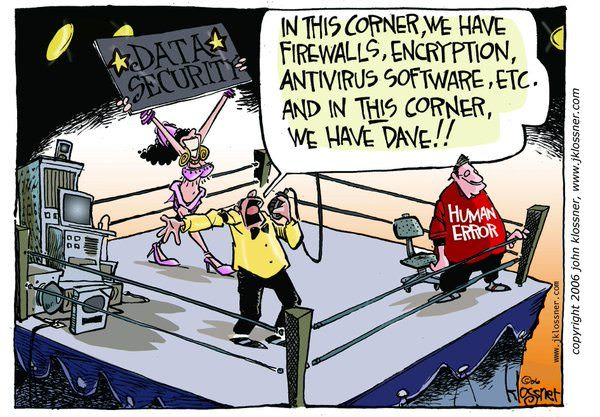
\includegraphics[width=.7\textwidth]{DaveSecurity}
\caption{Network Security - the sad truth}
\label{fig:dave}
\end{center}
\end{figure}

Note that, likewise tables and listings, you shall not worry about where the figures are placed. Moreover, you should not add the file extension (LaTeX will pick the `best' one for you) or the figure path.
\include{Chapters/07-Conclusions}

%--------------------------------------------------------------
% Bibliography
%--------------------------------------------------------------
\nocite{*} % Remove or comment this row to show in bibliography just the cited sources
\printbibliography

%--------------------------------------------------------------
\end{document}
%--------------------------------------------------------------
